\documentclass{article}
% Packages start
\usepackage{graphicx} 
\usepackage[italian]{babel}
\usepackage{algorithm2e}
\usepackage{amsthm}
\usepackage{algpseudocode}
\usepackage{float}
\usepackage{graphicx} %package to manage images
\usepackage{imakeidx}
\usepackage{amsmath}
% Packages end
%document data def start
\title{Intelligenza artificiale}
\author{Valerio Tolli}
\date{November 2024}
%document data def end
%theorem def start
\newtheorem{theorem}{Theorem}[subsection]
\newtheorem{lemma}{Lemma}[subsection]
%theorem def end
%document begin
\begin{document}
%indice start
\maketitle
\newpage
\tableofcontents
%indice end

%Cap. Introduzione start
\newpage
\section{Introduzione}
%Cap. Introduzione end

%Cap. Agenti intelligenti start
\newpage
\section{Agenti intelligenti}
%Agenti e ambiente start
\subsection{Agenti e ambiente}
\textbf{Definizione di agente:} Un agente è qualsiasi cosa possa essere vista come un sistema che percepisce il suo ambiente attraverso dei sensori e agisce su di esso mediante attuatori.\newline

\begin{figure}[H]
    \centering
    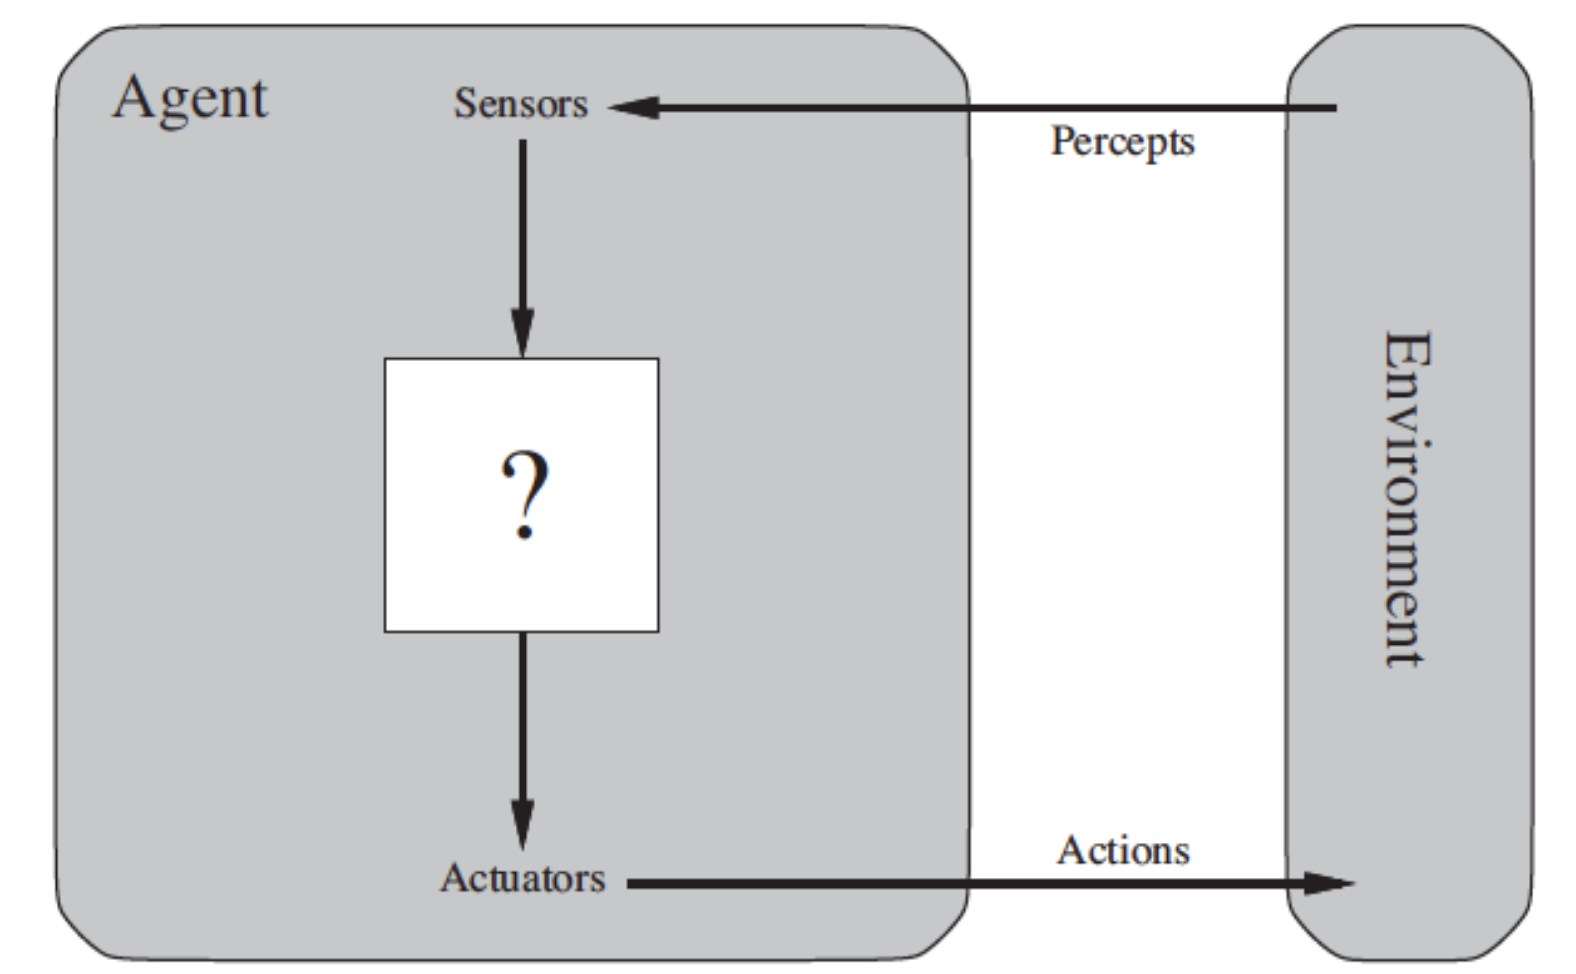
\includegraphics[width=0.5\linewidth]{Images/agenteBase.png}
    \caption{Agente}
    \label{fig:enter-label}
\end{figure}
\par\noindent\rule{\textwidth}{0.4pt}
\noindent\textbf{Esempi:}
\begin{itemize}
    \item Agente umano possiede sensori come occhi, orecchie, ecc…
    \item Agente software riceve come input sensori che possono essere dati, input umani, ecc…
\end{itemize}
\par\noindent\rule{\textwidth}{0.4pt}
\noindent Con il termine \textbf{percezione} si indicano i dati che i sensori di un agente percepiscono. La \textbf{sequenza percettiva} di un agente è la storia completa di tutto ciò che esso ha percepito nella sua esistenza.
In generale, la scelta dell'azione di un agente in un qualsiasi istante può dipendere dalla conoscenza integrata in esso e dall'intera sequenza percettiva osservata fino a quel momento, ma non da qualcosa che non abbia percepito.
Il comportamento di un agente è quindi descritto dalla \textbf{funzione agente}, che descrive l'azione da compiere per ogni sequenza percettiva.
Internamente, la funzione agente di un agente artificiale sarà implementata da un \textbf{programma agente}.  La funzione agente è una descrizione matematica astratta; il programma agente è la sua implementazione concreta, in esecuzione su un sistema fisico.
\par\noindent\rule{\textwidth}{0.4pt}
\noindent\textbf{Esempio: }Consideriamo l'agente aspirapolvere che percepisce lo sporco nel riquadro in cui si trova Una funzione agente può essere: "Se il riquadro corrente è sporco, aspira, altrimenti muoviti in un altro riquadro".
\par\noindent\rule{\textwidth}{0.4pt}
\noindent Un \textbf{agente razionale} è un agente che interagisce con il suo ambiente in maniera efficace, ovvero fa la cosa giusta: valutiamo il comportamento di un agente considerandone le conseguenze. Quando un agente viene inserito in un ambiente, genera un sequenza di azioni in base alle percezioni che riceve. Questa sequenza di azioni porta l'agente ad attraversare una \textbf{sequenza di stati}; se tale sequenza è \textbf{desiderabile} significa che l'agente si è comportato bene.\newline
Questa nozione di desiderabilità porta a imporre un criterio di valutazione oggettivo dell'effetto delle azioni dell'agente: ovvero serve una \textbf{misura di prestazione} che valuta una sequenza di stati dell'ambiente. La misura di prestazione per un agente artificiale è scelta dal progettista a seconda del problema considerando un'evoluzione desiderabile del mondo. In generale, è meglio progettare le misure di prestazione in base all'effetto che si desidera ottenere sull'ambiente piuttosto che su come si pensa che debba comportarsi l'agente.\newline

\noindent In un dato momento ciò che è razionale dipende da quattro fattori:
\begin{itemize}
    \item La misura di prestazione che definisce il criterio del successo;
    \item La conoscenza pregressa dell'ambiente da parte dell'agente;
    \item Le azioni che l'agente può effettuare;
    \item La sequenza percettiva dell'agente fino all'istante corrente.
\end{itemize}
\textbf{Definizione di agente razionale: }Per ogni possibile sequenza di percezioni, un agente razionale dovrebbe scegliere un'azione che massimizzi il valore atteso della sua misura di prestazione, date le informazioni fornite dalla sequenza percettiva e da ogni ulteriore conoscenza dell'agente.
\par\noindent\rule{\textwidth}{0.4pt}
\textbf{Esempio: }L'agente aspirapolvere per essere razionale bisogna prima di tutto definire la sua misura di prestazione, supponiamo che:
\begin{itemize}
    \item la misura di prestazione assegni un punto per ogni passo temporale, per una vita dell'agente di 1000 passi;
    \item sia nota a priori la geografia dell'ambiente, ma non la posizione iniziale dell'agente; le azioni destra-sinistra muovono l'agente di un riquadro nelle corrispondenti direzioni, e l'aspirazione dello sporco pulisce solo il riquadro corrente;
    \item le azioni disponibili sono Destra, Sinistra e Aspira;
    \item l'agente percepisce correttamente la propria posizione e se il riquadro corrente è sporco o meno.
\end{itemize}
\noindent Date queste condizioni, l'agente è razionale, le sue prestazioni sono buone almeno quanto quelle di qualsiasi altro agente.
\par\noindent\rule{\textwidth}{0.4pt}
%Agenti e ambiente end
%OAA start
\subsection{Onniscienza, apprendimento e autonomia}
Un agente onnisciente conosce il risultato effettivo delle sua azioni e può agire di conseguenza, ma nella realtà l'onniscienza è impossibile.\\
La razionalità quindi non è perfezione, la razionalità è massimizzare il risultato atteso, mentre la perfezione massimizza quello reale.\\
Una parte importante della razionalità è l'information gathering (raccolta di informazioni) ovvero intraprendere azioni mirate a modificare le percezioni future. \\
\par\noindent\rule{\textwidth}{0.4pt}
\textbf{Esempio: }un agente aspirapolvere che apprende come predire quando e dove apparirà lo sporco si comporterà meglio degli altri.
\par\noindent\rule{\textwidth}{0.4pt}
Un agente razionale oltre a raccogliere informazioni deve anche essere in grado di apprendere il più possibile sulla base delle proprie percezioni.\\ 
Un agente può anche appoggiarsi alla conoscenza pregressa fornita dal progettista invece che alle proprie percezioni e ai suoi processi di apprendimento, in questo caso si dice che manca di autonomia. Mentre un agente è autonomo quando il suo comportamento dipende dalla sua esperienza. \\
Per un agente di intelligenza artificiale è ragionevole fornire un po' di conoscenza pregressa e dopo aver accumulato una sufficiente esperienza in un dato ambiente può diventare indipendente dalla conoscenza pregressa.
%OAA end
%NaturaAmbienti start
\newpage
\subsection{La natura degli ambienti}
Gli ambienti operativi sono i problemi di cui gli agenti razionali rappresentano le soluzioni. I problemi possono essere descritti come PEAS (Performance, Environment, Actuators, Sensors).\newline
\textbf{Esempio agente guidatore di taxi:}
\begin{figure}[H]
    \centering
    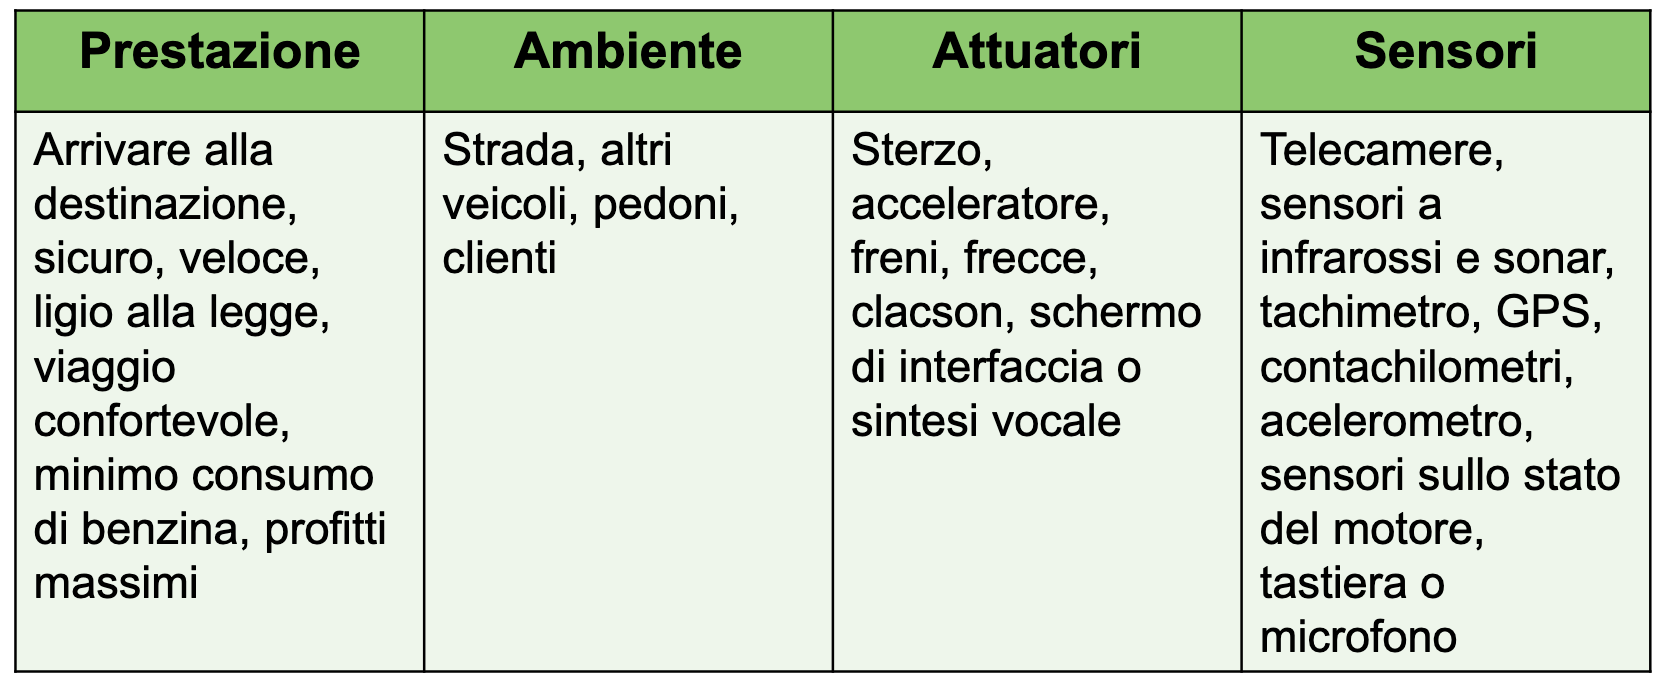
\includegraphics[width=0.5\linewidth]{Images/guidatoreTaxiPEAS.png}
    \caption{PEAS, agente guidatore di taxi}
    \label{fig:enter-label}
\end{figure}
\textbf{Esempi di tipi di agente e loro descrizioni PEAS:}
\begin{figure}[H]
    \centering
    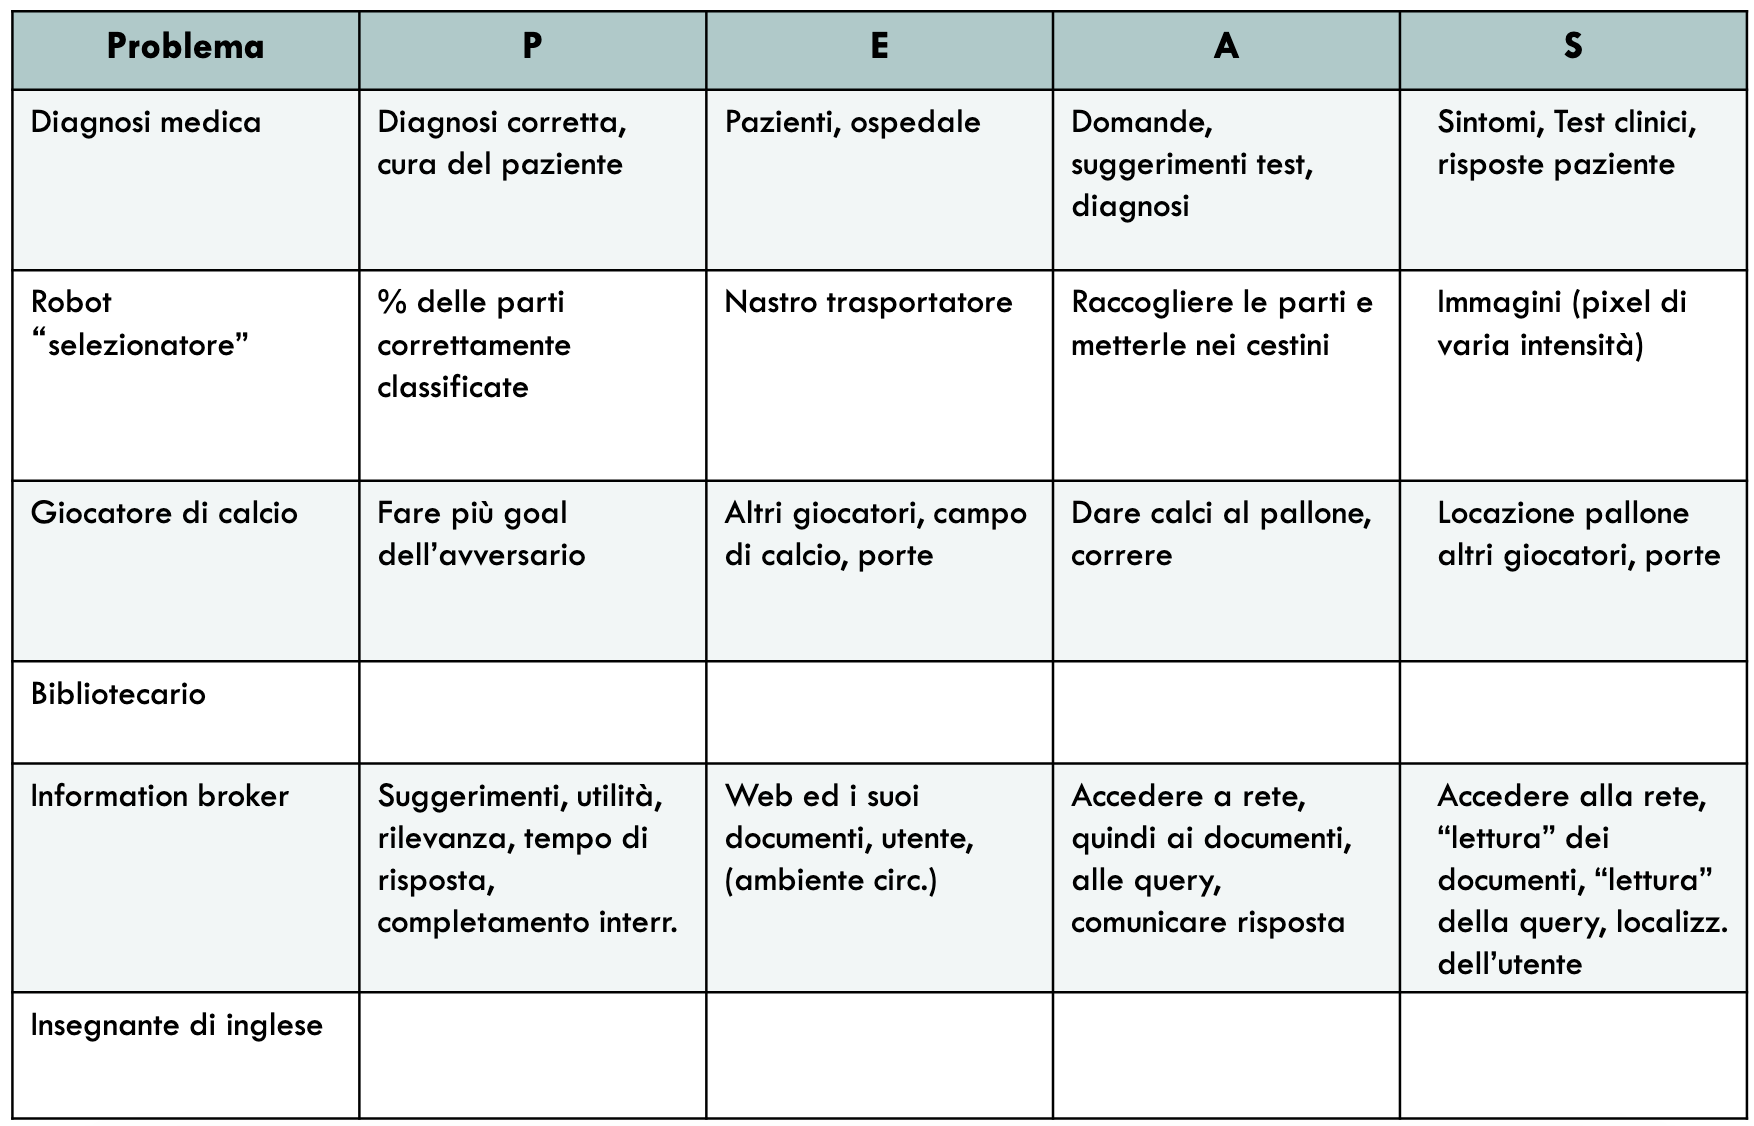
\includegraphics[width=0.5\linewidth]{Images/EsempiPEAS.png}
    \caption{Esempi PEAS}
    \label{fig:enter-label}
\end{figure}
\textbf{Proprietà degli ambienti operativi:}
\begin{itemize}
    \item \textbf{Completamente osservabile/ parzialmente osservabile: }Se i sensori dell'agente gli danno accesso allo stato completo dell'ambiente in ogni momento, allora diciamo che l'ambiente operativo è completamente osservabile.\\
    Per far ciò basta che i sensori dell'agente misurino tutti gli aspetti che sono rilevanti per la scelta dell'azione. La rilevanza dipende dalla misura di prestazione.\\
    Un ambiente si dice parzialmente osservabile o a causa di sensori non adeguati o per la presenza di rumore o perché una parte dei dati non viene rilevata dai sensori.\\
    Se l'agente non dispone di sensori, l'agente si dice inosservabile.\\
    \textbf{Esempi: aspirapolvere/slide}
    \item \textbf{Agente singolo/multiagente: }un agente che risolve da solo un cruciverba è in un ambiente ad agente singolo, mentre un agente che gioca a scacchi si trova in un ambiente ad agenti multipli. I multi-agenti possono essere competitivi (spesso nell'ambiente competitivo, il comportamento randomizzato è razionale perché permette di evitare la predicibilità della mossa) o cooperativi (Comunicazione comportamento razionale).
    \item \textbf{Deterministico/non deterministico: }si dice deterministico se lo stato dell'ambiente è completamente determinato dallo stato corrente e dall'azione eseguita dall'agente (o dagli agenti).\\
    Un agente si dice non deterministico se gli stati possibili non corrispondono ad una specifica distribuzione di probabilità, ovvero non eventuali varie possibilità non sono quantificate.\\
    Un agente si dice stocastico se esistono elementi di incertezza con associata probabilità.
    \item \textbf{Episodico/sequenziale: }in un ambiente operativo episodico l'esperienza dell'agente è divisa in episodi atomici. In ogni episodio l'agente riceve una percezione e poi esegue una singola azione. In ambienti episodici non c'è bisogno di pianificare (esempio: molte attività di classificazione, come classificare gli item difettosi prodotti da una fabbrica). Negli ambienti sequenziali ogni decisione influenza le successive (esempio: scacchi o guida dei taxi).
    \item \textbf{Statico/dinamico: }se l'ambiente può cambiare mentre un agente sta decidendo come agire, allora diciamo che è dinamico per quell'agente; altrimenti diciamo che è statico. Mentre l'ambiente statico è più semplice da gestire perché non deve guardare il mondo mentre sceglie l'azione successiva e non si deve preoccupare del tempo impiegato, l'ambiente dinamico chiede continuamente all'agente quello che vuole fare e se questo non risponde in tempo, è come se non avesse agito. Se l'ambiente stesso non cambia al passare del tempo, ma la valutazione dell'agente si allora diciamo che l'ambiente è semi-dinamico. (esempi: guidate un taxi è dinamico, gli scacchi sono semi-dinamici, i cruciverba sono statici).
    \item \textbf{Discreto/Continuo: }la descrizione tra discreto e continuo si applica allo stato dell'ambiente, al modo in cui vengono gestiti tempo, percezione e azioni dell'agente (esempio: scacchi hanno un insieme discreto di percezioni e azioni; la guida del taxi stati e tempi variano nel continuo).
    \item \textbf{Noto/Ignoto: }si riferisce allo stato di conoscenza dell'agente circa le cifre fisiche dell'ambiente stesso. Se l'agente è ignoto, l'agente dovrà apprendere come funziona per poter prendere buone decisioni. La distinzione tra ambienti noti e ignoti non è identica a quella tra ambienti completamente osservabili e parzialmente osservabili.\\
    Infatti è possibile che un ambiente noto sia parzialmente osservabile (esempio: giochi di carte, il giocatore conosce le regole, ma non può vedere le carte che non sono ancora state girate). Viceversa un ambiente ignoto può essere completamente osservabile (in un nuovo videogioco, un giocatore potrebbe non conoscere tutte le funzioni mostrate a schermo). Il caso più complesso è quello degli ambienti "reali" (in genere): parzialmente osservabili, stocastici, sequenziali, dinamici, continui, multi-agente, ignoti.
\end{itemize}
\textbf{Esempi:}
\begin{figure}[H]
    \centering
    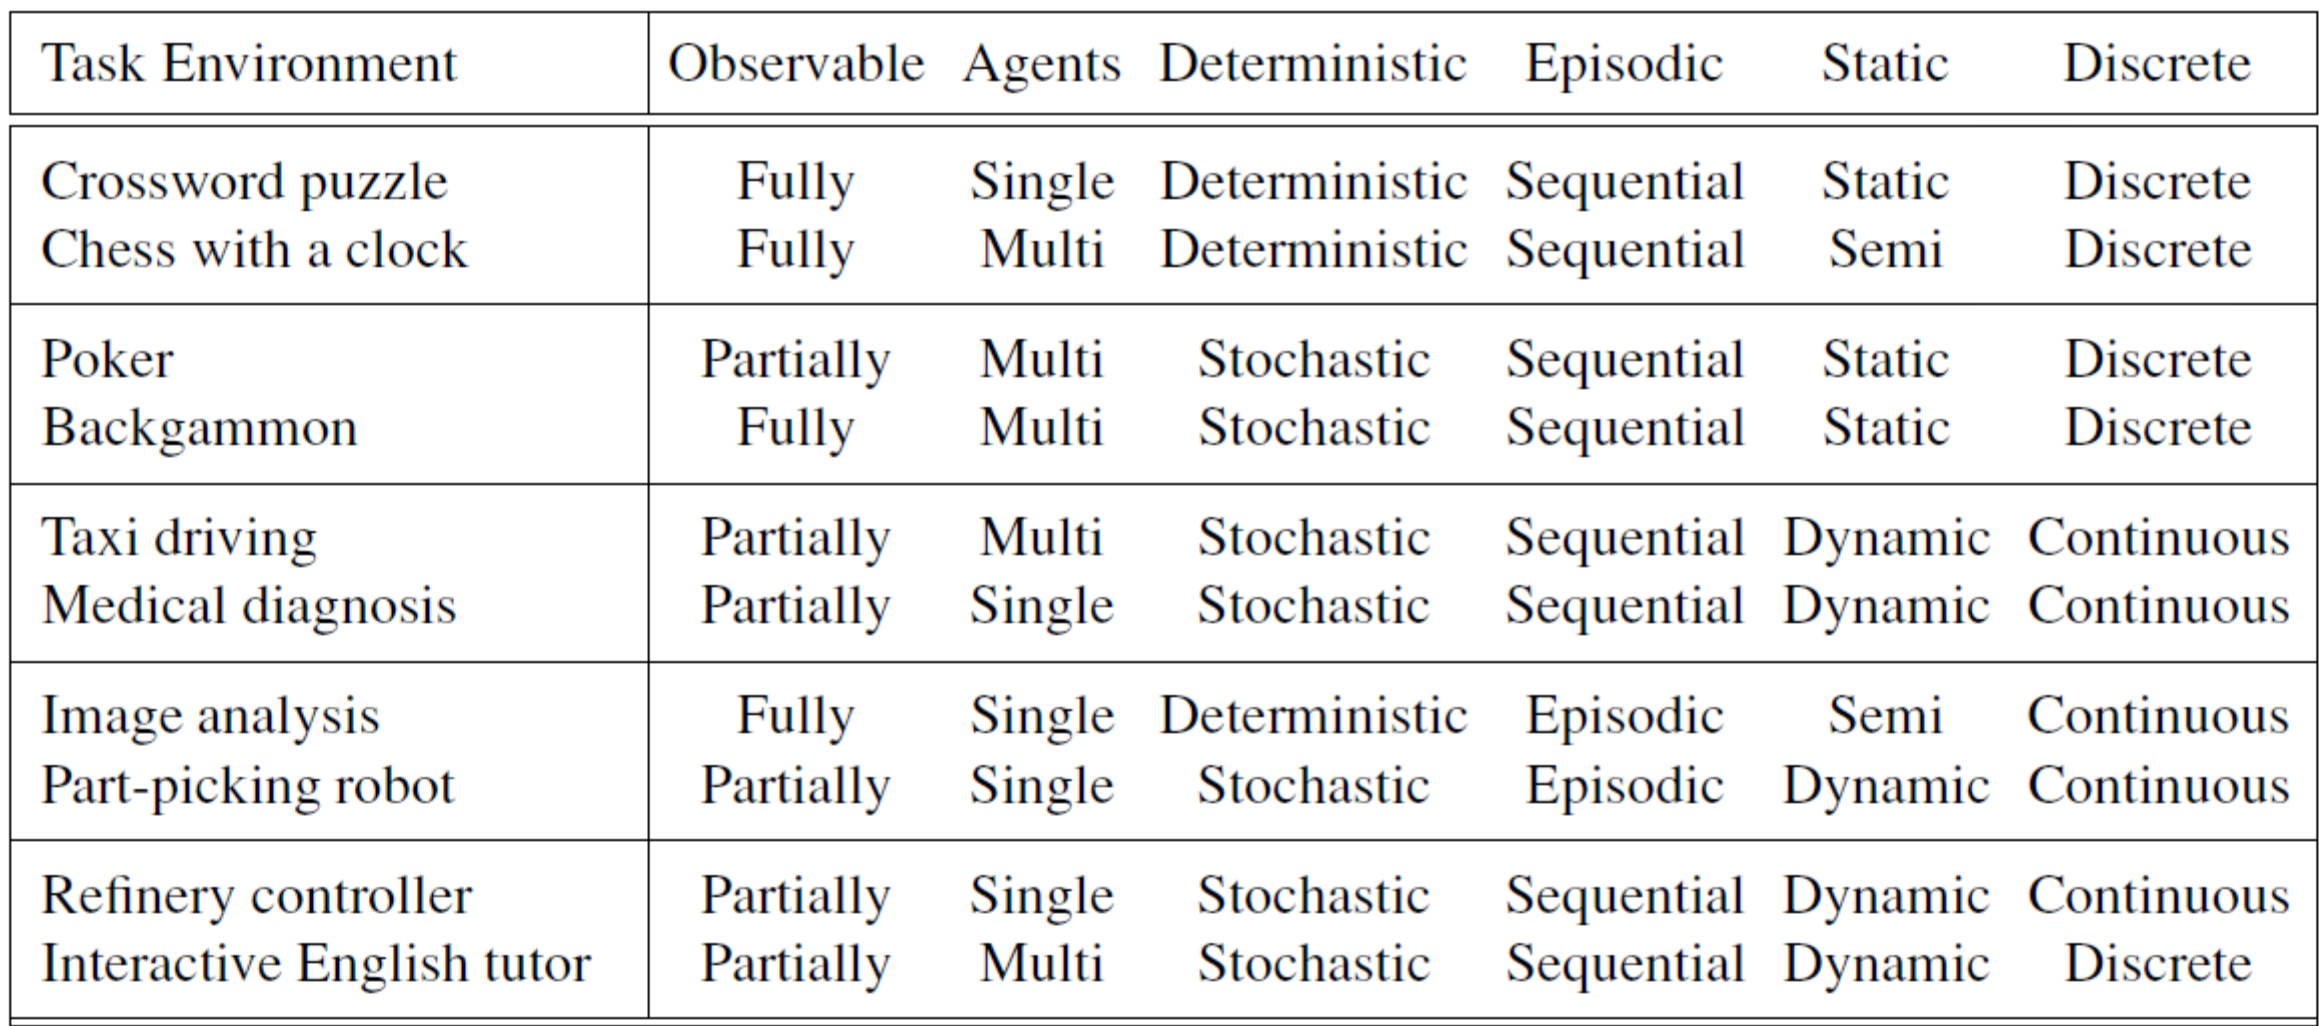
\includegraphics[width=0.5\linewidth]{Images/EsempiAmbiente.png}
    \caption{Esempi ambiente}
    \label{fig:enter-label}
\end{figure}
%NaturaAmbienti end
%La struttura degli agenti start
\newpage
\subsection{La struttura degli agenti}
\noindent Il compito della IA è progettare il programma agente che implementa la funzione agente che fa corrispondere le percezioni alle azioni. Diamo per scontato che questo programma sarà eseguito da un dispositivo computazionale dotato di sensori e attuatori fisici; questa prende il nome di architettura agente:\newline
\begin{center}
     agente = architettura + programma.
\end{center}
%La struttura degli agenti end
%programma agente start
\subsection{Programma Agente}
I programmi agente (che vedremo) hanno tutti la stessa struttura: prendono in input la percezione corrente dei sensori e restituiscono un'azione agli attuatori. La funzione agente invece potrebbe dipendere dall'intera storia delle percezioni.\newline

\par\noindent\rule{\textwidth}{0.4pt}
\noindent Esempio di un programma agente che viene eseguito per ogni nuova percezione e restituisce ogni volta l'azione da eseguire. Mantiene in memoria la sequenza percettiva completa:
%%%%%%%%%% funzione agente  start 
\begin{center}
\SetKwComment{Comment}{/* }{ */}
\begin{algorithm}
\caption{Funzione agente}
\KwData{percezione}
\KwResult{\Return un'azione;}
\textbf{persistent: }percezioni, una sequenza inizialmente vuota; tabella, una tabella di azioni indicizzata per sequenze percettive completamente specificata dall'inizio\;
aggiungi percezione alla fine di percezioni\;
$azione \leftarrow LOOKUP(percezioni, tabella)$\;
\Return azione\;
\end{algorithm}
\end{center}
%%%%%%%%%% funzione agente  end
\par\noindent\rule{\textwidth}{0.4pt}
\noindent Negli agenti con tabella viene costruita una tabella che contiene l'azione appropriata per ogni possibile sequenza percettiva.
Questo approccio è estremamente fallimentare:
Consideriamo l'insieme delle percezioni P e sia T la durata di vita dell'agente; la tabella conterrà $\sum_{t=1}^n|P|^t$ righe.
%programma agente end
%Agenti reattivi semplici start
\newpage
\subsection{Agenti reattivi semplici}
Scelgono le azioni sulla base della percezione corrente, ignorando la storia percettiva precedente (esempio l'aspirapolvere è un agente reattivo semplice).
\par\noindent\rule{\textwidth}{0.4pt}
\noindent Esempio di programma agente per l'agente reattivo semplice nell'ambiente dell'aspirapolvere a due stati.
%%%%%%%%%% funzione agente  start 
\begin{center}
\SetKwComment{Comment}{/* }{ */}
\begin{algorithm}
\caption{Agente-Reattivo-Aspirapolvere}
\KwData{[posizione,stato]}
\KwResult{\Return un'azione;}
\If{stato = sporco}{\Return Aspira}
{\If{posizione = A}{\Return Destra}}
{\If{posizione = B}{\Return Sinistra}}
\end{algorithm}
\end{center}
%%%%%%%%%% funzione agente  end
\par\noindent\rule{\textwidth}{0.4pt}
\begin{figure}[H]
    \centering
    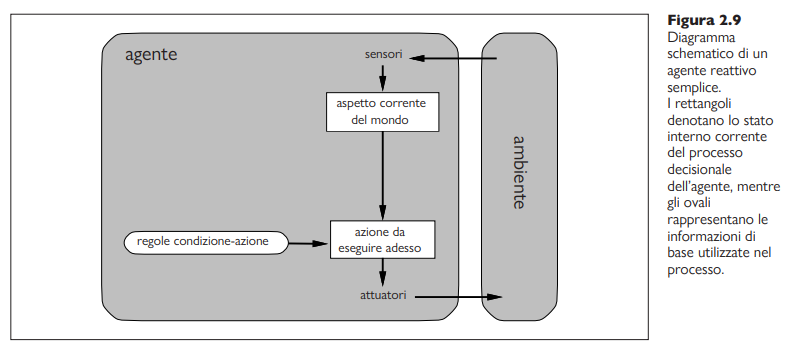
\includegraphics[width=0.5\linewidth]{Images/diagrammaAgenteReattivoSemplice.png}
    \caption{Diagramma schematico di un agente reattivo semplice}
    \label{fig:enter-label}
\end{figure}
\par\noindent\rule{\textwidth}{0.4pt}
\noindent Esempio di programma agente per l'agente reattivo semplice che agisce secondo una regola la cui condizione corrisponde allo stato corrente, indicato dalla percezione. INTERPRETA-INPUT genera una descrizione astratta dello stato corrente partendo dalla percezione; REGOLA-CORRISPONDENTE restituisce la prima regola dell'insieme che corrisponde a tale descrizione.
%%%%%%%%%% Agente-Reattivo-Semplice  start 
\begin{center}
\SetKwComment{Comment}{/* }{ */}
\begin{algorithm}
\caption{Agente-Reattivo-Semplice}
\KwData{percezione}
\KwResult{\Return un'azione;}
\textbf{persistent: }regole, un insieme di regole condizione-azione\;
$stato \leftarrow INTERPRETA-INPUT(percezione)$\;
$regola \leftarrow REGOLA_CORRISPONDENTE(stato, regole)$\;
$azione \leftarrow regola.AZIONE$\;
\Return azione
\end{algorithm}
\end{center}
\par\noindent\rule{\textwidth}{0.4pt}
%%%%%%%%%% Agente-Reattivo-Semplice end
Questo agente funziona solo se si può selezionare la decisione corretta in base alla sola percezione corrente, ovvero solo nel caso in cui l'ambiente sia completamente osservabile.\newline
\noindent Per evitare che gli agenti caschino in cicli infiniti, soprattutto quelli con limitate percezioni, è utile randomizzare le sue azioni scegliendone una in modo casuale.\newline
\noindent Esempio, se l'aspirapolvere percepisce Pulito, allora si sposta a Destra o Sinistra in modo casuale. In genere negli ambienti ad agente singolo la randomizzazione non è razionale, può aiutare gli agenti reattivi semplici a districarsi da certe situazioni, ma spesso è meglio ricorrere ad agenti più sofisticati.
%Agenti reattivi semplici end
%Agenti reattivi basati su modello start
\newpage
\subsection{Agenti reattivi basati su modello}
Il modo più generale di gestire l'osservabilità parziale è tenere uno stato interno all'agente che dipende dalla storia delle percezioni e che quindi riflette almeno una parte degli aspetti non osservabili dello stato corrente. Per aggiornare lo stato interno l'agente deve avere due tipi di informazioni:
\begin{itemize}
    \item Informazioni sull'evoluzione del mondo nel tempo, che sono suddivisibili in due parti: gli effetti delle azioni dell'agente sul mondo e le modalità di evoluzione del mondo indipendenti dall'agente. Questa conoscenza sul funzionamento del mondo si chiama \textbf{modello di transizione del mondo}.
    \item Informazioni su come lo stato del mondo si riflettano nelle percezioni dell'agente, chiamata \textbf{modello sensoriale}.
\end{itemize}
\noindent Il modello di trasmissione e il modello sensoriale consentono all'agente di tenere traccia dello stato del mondo (considerando le limitazioni dei sensori); un agente che utilizza tali sensori prende il nome di agente basato su modello.
\begin{figure}[H]
    \centering
    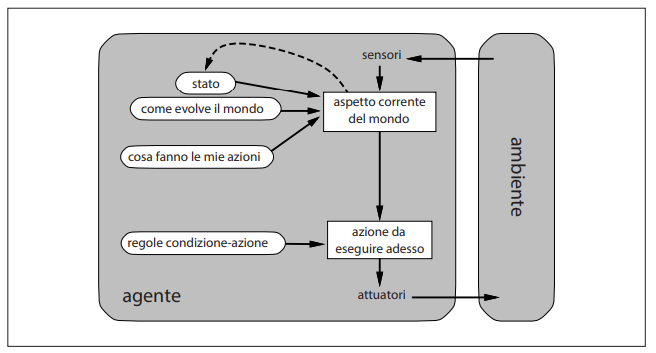
\includegraphics[width=0.5\linewidth]{Images/AgenteReattivoBasatoSuModello.png}
    \caption{Diagramma agente reattivo basato su modello}
    \label{fig:enter-label}
\end{figure}
\par\noindent\rule{\textwidth}{0.4pt}
\noindent Esempio di programma agente per l'agente reattivo basato su modello. La funzione AGGIORNA-STATO è responsabile della creazione del nuovo stato interno.
%%%%%%%%%% Agente-Reattivo-Basato-su-modello start 
\newpage
\begin{center}
\SetKwComment{Comment}{/* }{ */}
\begin{algorithm}
\caption{Agente-Reattivo-Basato-Su-Modello }
\KwData{percezione}
\KwResult{\Return un'azione;}
\textbf{persistent: }\textit{stato}, la concezione corrente dello stato del mondo da parte dell'agente;\newline
\textit{modello\_transizione}, una descrizione della dipendenza dello stato successivo dallo stato corrente e dall'azione;\newline
\textit{modello\_sensoriale}, una descrizione di come lo stato del mondo attuale è riflesso nelle percezioni dell'agente;\newline
\textit{regole}, un insieme di regole condizione-azione;\newline
\textit{azione}, l'azione più recente, inizialmente nessuna\;
\textit{stato} $\leftarrow$ AGGIORNA-STATO(stato, azione, percezione, modello\_transizione, modello\_sensoriale)\;
\textit{regola} $\leftarrow$ REGOLA-CORRISPONDENTE(stato,regole)\;
\textit{azione} $\leftarrow$ \textit{regola}.AZIONE\;
\Return azione
\end{algorithm}
\end{center}
\par\noindent\rule{\textwidth}{0.4pt}
%%%%%%%%%% Agente-Reattivo-Basato-su-modello end
%Agenti reattivi basati su modello end
%Agenti basati su obiettivi start
\newpage
\subsection{Agenti basati su obiettivi}
Non sempre basta lo stato corrente per decidere cosa fare. In alcuni casi l'agente deve conoscere le informazioni riguardante il suo obiettivo (goal). Un agente basato su obiettivi ha un programma agente che unisce queste informazioni al modello. Per raggiungere questi obiettivi vengono applicate ricerche e pianificazione (verranno approfondite in seguito).
A differenza degli agenti reattivi dove le azioni sono rappresentate esplicitamente, un agente basato su obiettivi esegue determinate azioni perché, secondo la sua previsione, permettono di raggiungere un determinato obiettivo.
Un'agente basato su obiettivi è meno efficace, ma più flessibile perché la conoscenza che guida le sue decisioni è rappresentata esplicitamente e può essere modificata.
\begin{figure}[H]
    \centering
    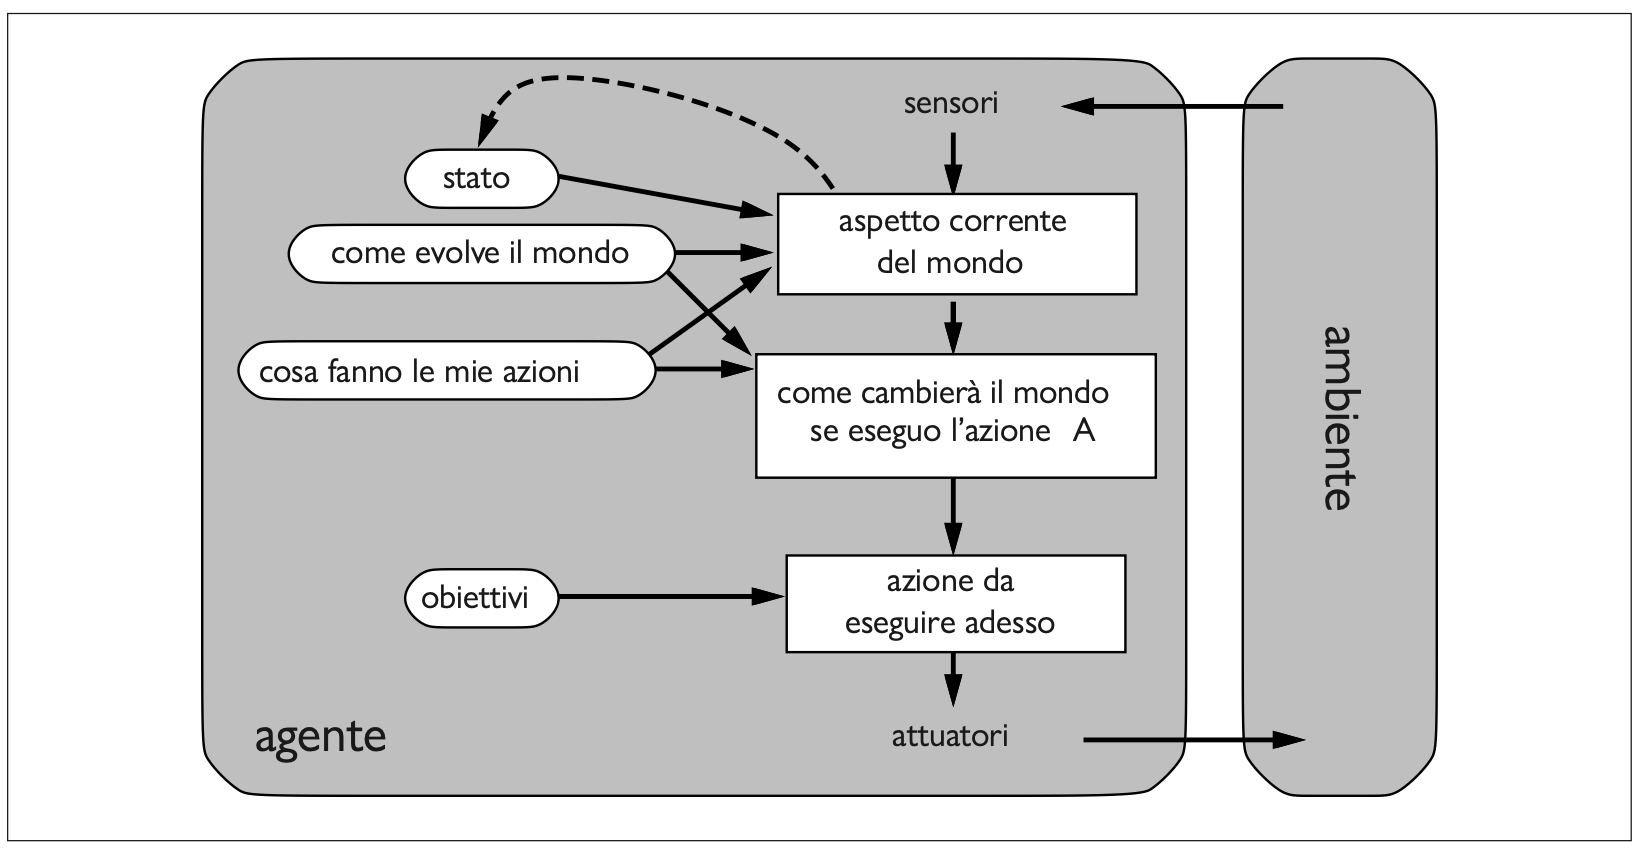
\includegraphics[width=0.5\linewidth]{Images/AgenteBasatoObiettivi.png}
    \caption{Diagramma Agente basato su obiettivi}
    \label{fig:enter-label}
\end{figure}
%Agenti basati su obiettivi end
%Agenti basati sull'utilità start
\newpage
\subsection{Agenti basati sull'utilità}
In alcuni ambienti gli obiettivi non bastano a generare un comportamento di alta qualità. Gli agenti basati sull'utilità ha una \textbf{funzione di utilità} che è un'internalizzazione della funzione di prestazione, che associa un numero reale ad un obiettivo. Ci sono due casi dove gli obiettivi sono inadeguati, ma l'agente basati sull'utilità è in grado di prendere decisioni razionali:
\begin{itemize}
    \item Quando ci sono obiettivi in conflitti e non si possono soddisfare tutti insieme, la funzione di utilità specifica come bilanciarli.
    \item Quando ci sono più obiettivi da raggiungere, ma nessuno lo si può raggiungere con certezza, il concetto di utilità fornisce un mezzo per confrontare le probabilità di successo e l'importanza degli obiettivi.
\end{itemize}
\noindent Un agente basato sull'utilità sceglie l'azione che massimizza l'utilità attesa dei risultati, ovvero l'utilità che l'agente si attende di ottenere, in media, date le probabilità e le utilità di ciascun obiettivo.\newline
\noindent Un agente che possiede una funzione di utilità esplicita può prendere decisioni razionali, seguendo un algoritmo generale che non dipende dalla specifica funzione di utilità che si desidera massimizzare.\newline
\noindent Un agente basato sull'utilità deve modellare e tenere traccia del proprio ambiente, e questi compiti hanno comportato lunghe e approfondite ricerche su percezione, rappresentazione, ragionamento e apprendimento.
\begin{figure}[H]
    \centering
    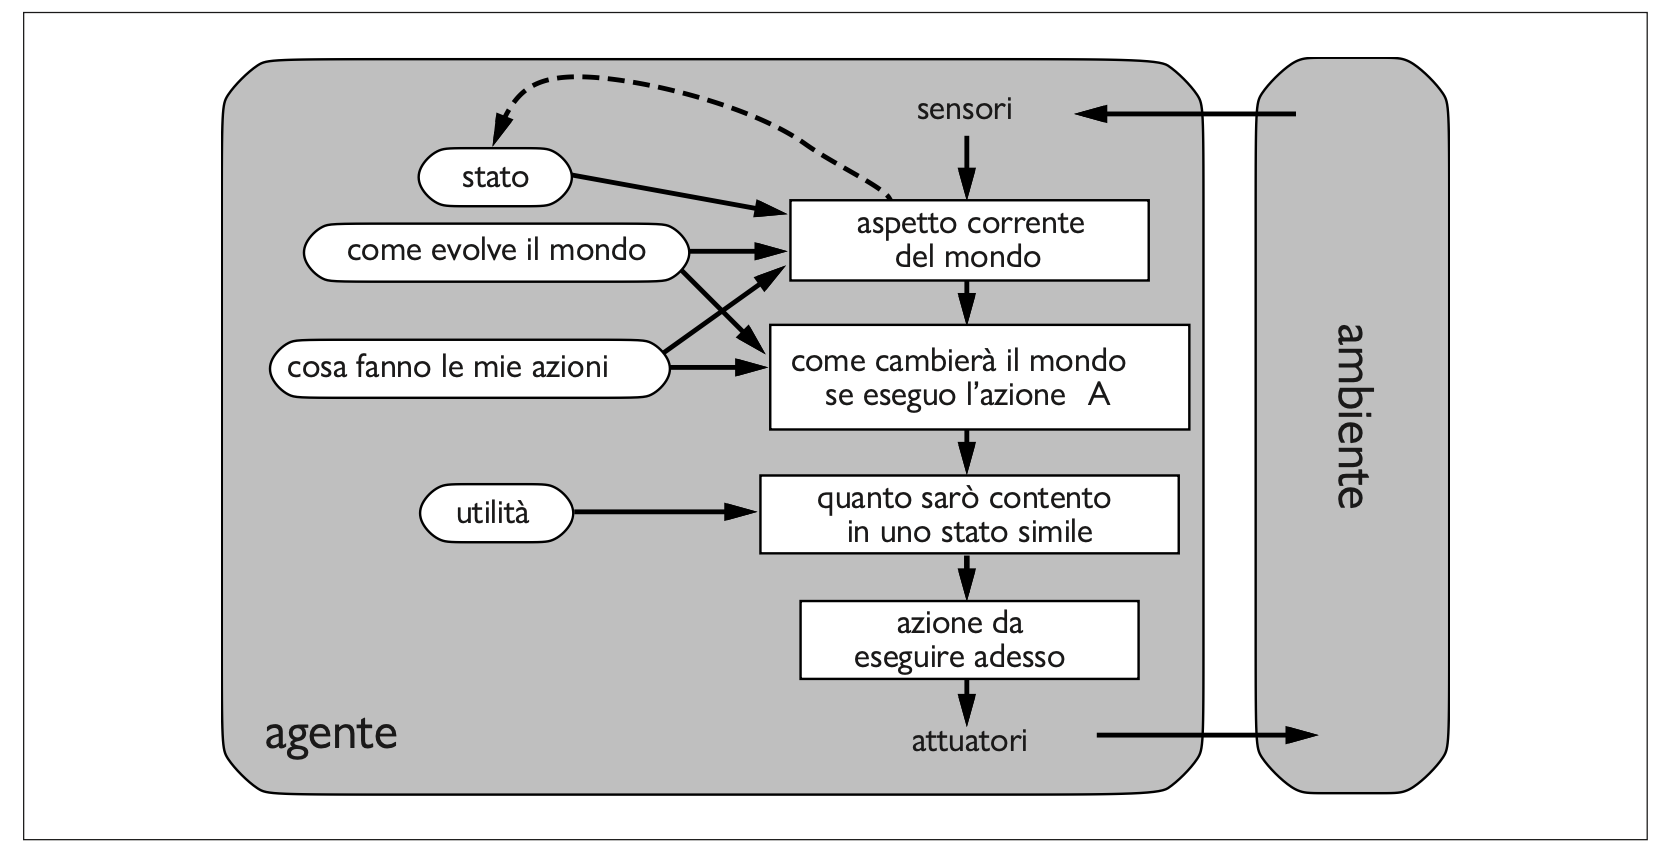
\includegraphics[width=0.5\linewidth]{Images/AgenteBasatoUtilita.png}
    \caption{Schema Agente basato sull'utilità}
    \label{fig:enter-label}
\end{figure}
%Agenti basati sull'utilità end
%Agenti capaci di apprendere start
\newpage
\subsection{Agenti capaci di apprendere}
Un agente capace di apprendere può essere diviso in quattro componenti astratti:
\begin{itemize}
    \item \textbf{Elemento di apprendimento}: responsabile del miglioramento interno e, in base alle informazioni ottenute dall'elemento critico, determina se e come modificare l'elemento esecutivo affinché nel futuro si comporti meglio;
    \item \textbf{Elemento esecutivo}: si occupa della selezione delle azioni esterne (ciò che fin ora abbiamo considerato l'intero agente). In fase di progettazione influenza il progetto dell'elemento di apprendimento;
    \item \textbf{Elemento critico}: fornisce informazioni all'elemento di apprendimento riguardo le prestazioni correnti dell'agente rispetto a uno standard prefissato.
    \item \textbf{Generatore di problemi}: suggerisce azioni che portino a esperienze nuove e significative. Questo fa si che invece di continuare ad eseguire le azioni migliori date le conoscenze attuali, vengano eseguite azioni sub-ottime nel breve termine, che nel lungo termine possano poi rilevarsi migliori.
\end{itemize}
\begin{figure}[H]
    \centering
    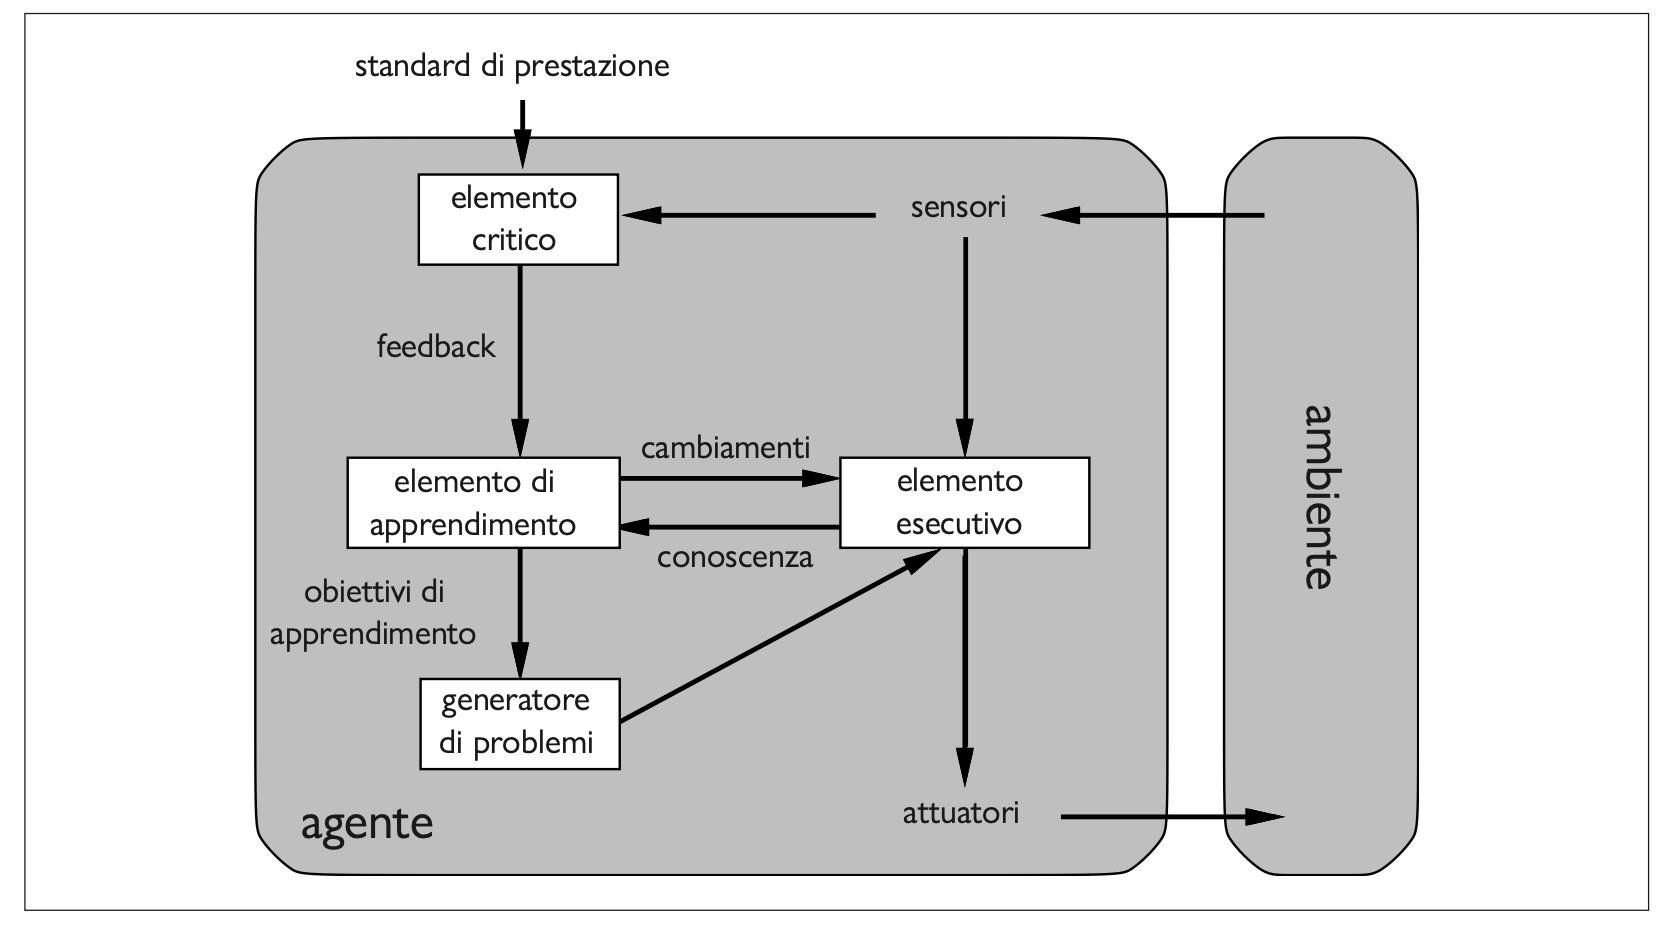
\includegraphics[width=0.5\linewidth]{Images/AgenteCapaceDiApprendere.png}
    \caption{Diagramma agente capace di apprendere}
    \label{fig:enter-label}
\end{figure}
%Agenti capaci di apprendere end
%Funzionamento dei comportamenti dei programmi agente start
\newpage
\subsection{Funzionamento dei comportamenti dei programmi agente}
Di seguito tre modi per rappresentare stati e transizioni fra loro:
\begin{itemize}
    \item \textbf{Rappresentazione atomica}: Ogni stato del mondo è indivisibile, non ha struttura interna. 
    \item \textbf{Rappresentazione fattorizzata}: suddivide ogni stato in un insieme fissato di variabili o attributi, ognuno dei quali può avere un valore. 
    \item \textbf{Rappresentazione strutturata}: descrive in modo esplicito oggetti (come mucche o camion) insieme alle loro relazioni. Sono alla base dei database relazionali e della logica del primo ordine, dei modelli probabilistici del primo ordine e LLM.
\end{itemize}
\begin{figure}[H]
    \centering
    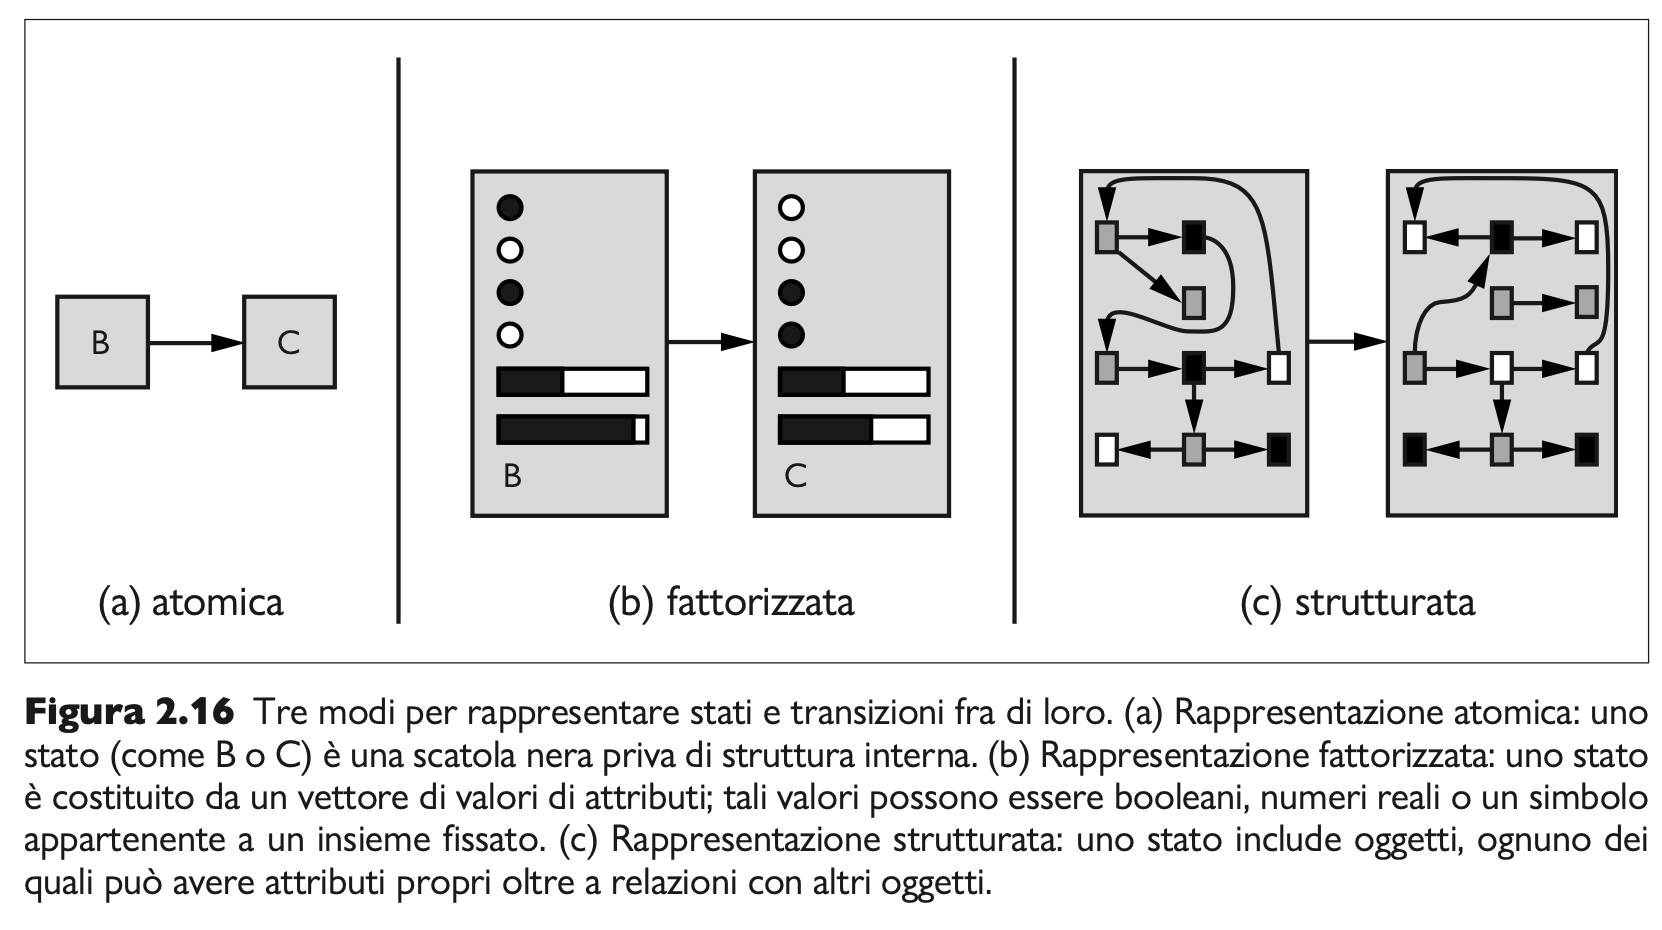
\includegraphics[width=0.5\linewidth]{Images/RappresentazioniStatiTransazioni.png}
    \caption{Rappresentazione di stati e transizioni}
    \label{fig:enter-label}
\end{figure}
Una rappresentazione più espressiva può catturare, con livello di concisione almeno uguale, tutto ciò che è in grado di catturare una rappresentazione meno espressiva.
%Funzionamento dei comportamenti dei programmi agente end
%Cap. Agenti intelligenti end
%Cap. Risolvere i problemi con la ricerca start
\newpage
\section{Risolvere i problemi con la ricerca}
%Agenti risolutori di problemi start 
\subsection{Agenti Risolutori di problemi}
Un agente risolutore di problemi è un agente che effettua azioni di ricerca. La ricerca deve essere effettuata su una sequenza di azioni che formano un cammino che porterà ad uno stato obiettivo. Essi utilizzano rappresentazioni atomiche in cui gli stati del mondo sono considerati come entità prive di una struttura interna visibile agli algoritmi per la risoluzioni dei problemi.
Supponiamo che i nostri agenti possano sempre avere accesso alle informazioni sul mondo, l'agente può eseguire un processo di risoluzione del problema in quattro fasi:
\begin{itemize}
    \item \textbf{Formulazione dell'obiettivo}: viene determinato un obiettivo (insieme di stati). Gli obiettivi aiutano a organizzare il comportamento limitando gli scopi e quindi le azioni da considerare.
    \item \textbf{Formulazione del problema}: l'agente elabora una descrizione degli stati e delle azioni necessarie per raggiungere l'obiettivo, ovvero un modello astratto della parte del mondo interessata.
    \item \textbf{Ricerca}: prima di effettuare qualsiasi azione nel mondo reale, l'agente simula più sequenze che non raggiungono l'obiettivo, ma alla fine troverà una soluzione, oppure troverà che non è possibile alcuna soluzione (esecuzione algoritmi di ricerca).
    \item \textbf{Esecuzione}: l'agente ora può eseguire le azioni specificate nella soluzione, una per volta.
\end{itemize}
Se l'ambiente è completamente osservabile, deterministico e noto, la soluzione di qualsiasi problema è una sequenza fissata di azioni. Se il modello è corretto, una volta che l'agente ha trovato una soluzione, può ignorare le sue percezioni mentre esegue le azioni dato che ha la garanzia che la soluzione lo condurrà all'obiettivo. 
Nella teoria del controllo si parla di anello aperto perché si rompe il ciclo tra agente e ambiente. Se vi è una possibilità che il modello sia errato o l'ambiente non deterministico, si parla di anello chiuso che tiene monitorate le percezioni.
%Agenti risolutori di problemi end
%Problemi di ricerca e soluzioni start
\newpage
\subsubsection{Problemi di ricerca e soluzioni}
Un problema di ricerca può essere definito formalmente come segue:
\begin{itemize}
    \item Un insieme di possibili stati in cui può trovarsi l'ambiente. Lo chiamiamo spazio degli stati.
	\item Lo stato iniziale in cui si trova l'agente inizialmente.
	\item Un insieme di uno o più stati obiettivo. A volte lo stato obiettivo è uno solo, a volte c'è un piccolo insieme di stati obiettivo alternativi, a volte l'obiettivo è definito da una proprietà che è soddisfatta da molti stati.
	\item Le azioni possibili dell'agente. Dato uno stato s, AZIONI(s) restituisce un insieme finito di azioni che possono essere eseguite in s. Diciamo che ognuna di queste azioni è applicabile in s.
	\item Un modello di transizione che descrive ciò che fa ogni azione. RISULTATO(s, a)restituisce lo stato risultante dell'esecuzione dell'azione a nello stato s.
	\item Una funzione di costo dell'azione, denotata da COSTO-AZIONE(s, a, s') o c(s, a, s') che restituisce il costo numerico di applicare l'azione a nello stato s per raggiungere s'.
\end{itemize}
Una sequenza di azioni forma un cammino; una soluzione è un cammino che porta dallo stato iniziale a uno stato obiettivo. Una soluzione ottima è, tra tutte le possibili soluzioni, quella con il costo minimo.
%Problemi di ricerca e soluzioni end
%Formulazione dei problemi start
\newpage
\subsubsection{Formulazione dei problemi}
Consideriamo il seguente problema: data questa mappa stradale trovare la miglior soluzione che ci possa portare da Arad a Bucarest
\begin{figure}[H]
    \centering
    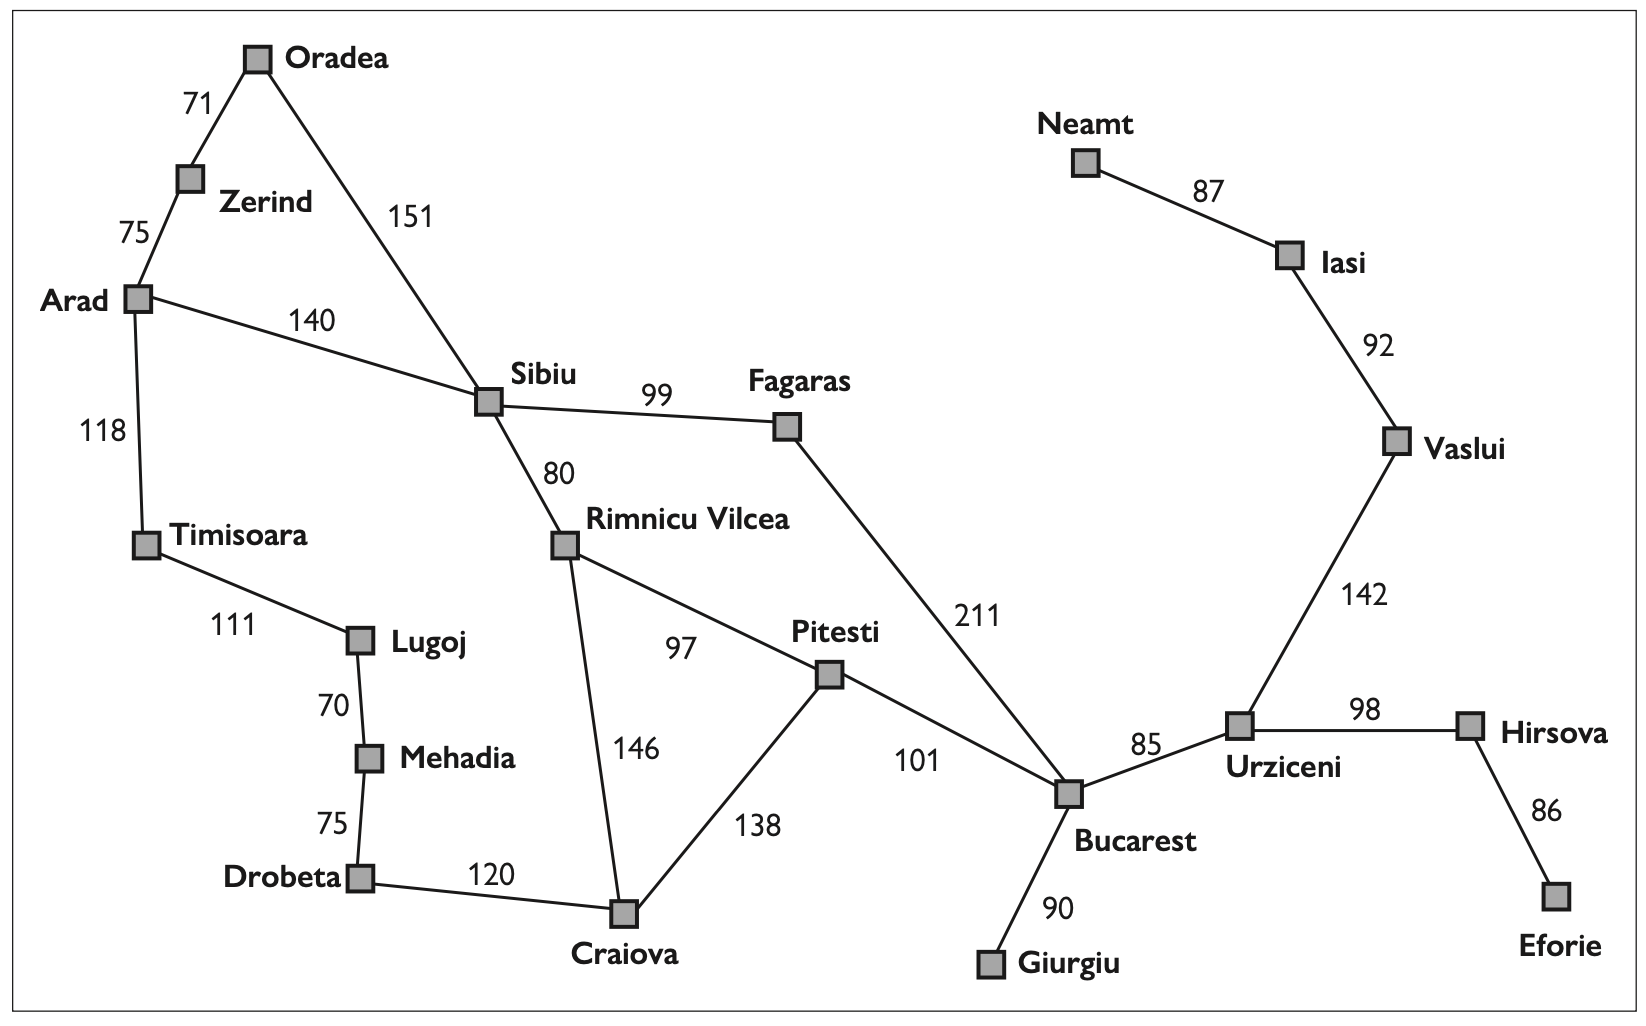
\includegraphics[width=0.5\linewidth]{Images/MappaStradaleRomania.png}
    \caption{Mappa Stradale Romania}
    \label{fig:enter-label}
\end{figure}
\noindent La nostra formulazione del problema di arrivare a Bucarest è un \textbf{modello}, cioè una descrizione matematica astratta, e non qualcosa di reale. Dal problema sono stati tolti tutti i dettagli inutili, questo processo prende il nome di \textbf{astrazione}. Un'astrazione è valida se possiamo espandere ogni soluzione astratta in una soluzione nel mondo più dettagliato.\newline


%Formulazione dei problemi end
%Problemi esemplificativi start
\newpage
\subsection{Problemi esemplificativi}
Lo scopo del \textbf{problema standardizzato} è illustrare o mettere alla prova diversi metodi di risoluzione di problemi. Può essere descritto in modo preciso e sintetico e quindi può essere usato come benchmark per confrontarne le prestazioni. Un \textbf{problema del mondo reale} è un problema le cui soluzioni sono effettivamente utili alle persone e la cui formulazione è specifica (esempio: problema del robot, dove ciascun robot è dotato di sensori diversi che producono dati diversi).
%Problemi esemplificativi end
%Problemi standardizzati start
\newpage
\subsubsection{Problemi standardizzati}
In un problema su griglia il mondo è una matrice bidimensionale costituita da un rettangolo di celle quadrate in cui gli agenti possono spostarsi da una cella all'altra.
\par\noindent\rule{\textwidth}{0.4pt}
\begin{figure}[H]
    \centering
    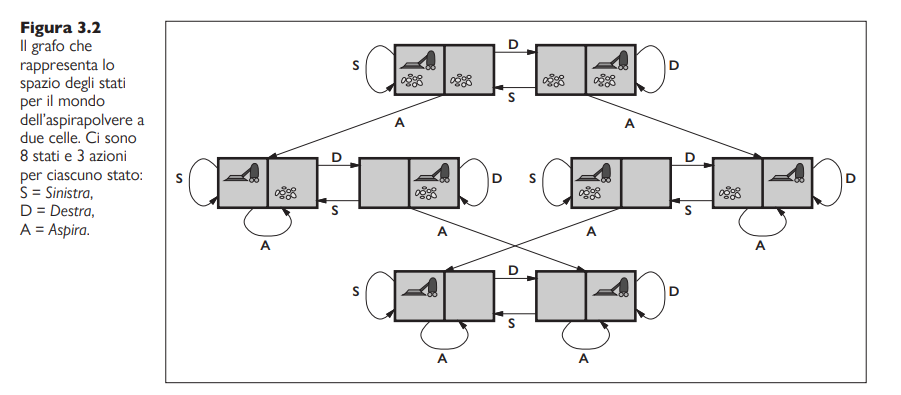
\includegraphics[width=0.5\linewidth]{Images/grafoSpazioStatiAspirapolvere.png}
    \caption{Grafo dello spazio degli stati per il mondo aspirapolvere a due celle}
    \label{fig:enter-label}
\end{figure}
Il mondo dell'aspirapolvere in figura può essere formulato come problema su griglia nel seguente modo:
\begin{itemize}
    \item \textbf{Stati}: uno stato del mondo indica quali oggetti sono in quali celle. Nel mondo dell'aspirapolvere gli oggetti sono l'aspirapolvere e lo sporco. Un mondo dell'aspirapolvere con n celle ha $n2^n$;
    \item \textbf{Stato iniziale}: ogni stato può essere designato come stato obiettivo;
    \item \textbf{Azioni}: In un mondo a due celle abbiamo: Sinistra, Destra, Aspira. In un mondo con n celle potremmo avere più stati, come: Su, Giù, … dette azioni di movimento assolute o azioni egocentriche come: Avanti, Indietro, Gira-A-Destra, … (dal punto di vista dell'agente);
    \item \textbf{Modello di transizione}: l'azione Aspira rimuove lo sporco dalla cella dove si trova l'agente; Avanti muove l'agente di una cella nella direzione verso cui è orientato;
    \item Stati obiettivo: gli stati in cui ogni cella è pulita;
    \item Costo di azione: ogni azione costa 1.
\end{itemize}
\par\noindent\rule{\textwidth}{0.4pt}
\begin{figure}[H]
    \centering
    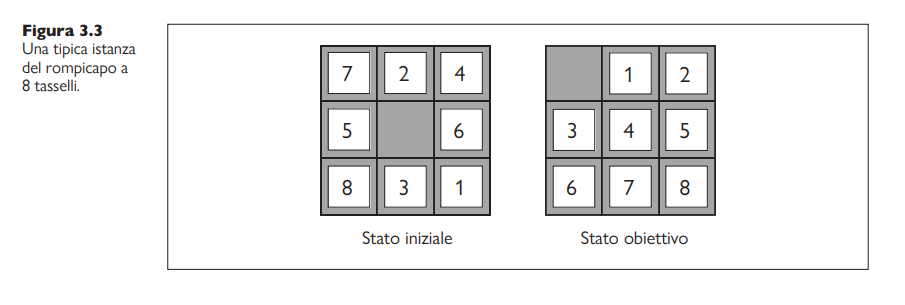
\includegraphics[width=0.5\linewidth]{Images/rompicapoSokoban8Tasselli.png}
    \caption{Rompicapo Sokoban a 8 tasselli}
    \label{fig:enter-label}
\end{figure}
\textbf{Esempio} rompicapo sokoban (generalizzazione del gioco dell'otto) ad otto tasselli:
\begin{itemize}
    \item Stato: una descrizione di stato specifica la posizione di ognuno degli otto tasselli;
    \item Stato iniziale: ogni stato può essere designato come stato iniziale;
    \item Azioni: descriviamo il movimento dello spazio vuoto, che può muoversi a Sinistra, Destra, Su o Giù. Se lo spazio vuoto si trova in un bordo o nell'angolo, no tutte le direzioni sono disponibili;
    \item Modello di transizione: fa corrispondere a uno stato e un'azione lo stato risultante; se ad esempio applichiamo un azione sulla casella vuota, essa prevede che la casella cambierà di posto con un'altra casella;
    \item Stato obiettivo: ogni stato potrebbe essere quello obiettivo, spesso viene specificato uno stato con i numeri ordinati (come in figura);
    \item Costo di azione: ogni azione costa 1.
\end{itemize}
\par\noindent\rule{\textwidth}{0.4pt}
\begin{figure}[H]
    \centering
    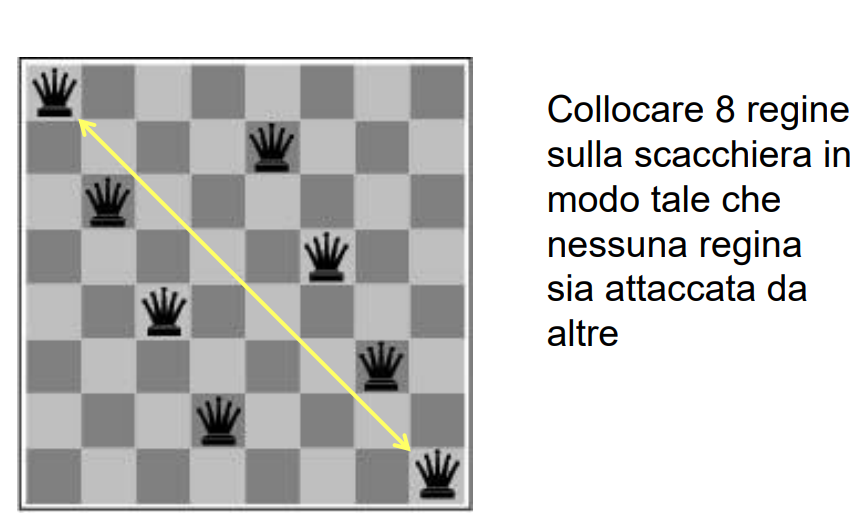
\includegraphics[width=0.5\linewidth]{Images/problema8Regine.png}
    \caption{Problema delle otto regine}
    \label{fig:enter-label}
\end{figure}
\textbf{Problema delle otto regine:}
\begin{itemize}
    \item Stati: scacchiera con 0-8 regine, nessuna minacciata;
    \item Stato iniziale: scacchiera vuota;
    \item Azioni: sposta una regina nella colonna, se minacciata;
    \item Stato obiettivo: 8 regine sulla scacchiera, nessuna minacciata;
    \item Costo di azione: ogni azione costa 0.
\end{itemize}
\par\noindent\rule{\textwidth}{0.4pt}
%Problemi standardizzati end
%Problemi reali start
\newpage
\subsubsection{Problemi reali}
Consideriamo il problemi di viaggio aereo che devono essere risolti da un sito web per la pianificazione dei viaggi:
\begin{itemize}
    \item Stati: ognuno comprende una posizione (un aeroporto) e l'ora corrente. Inoltre, poiché il costo di un'azione può dipendere da eventuali tratte precedenti, dalle loro tariffe e dal loro stato di tratte nazionali o internazionali, lo stato deve registrare altre informazioni su questi aspetti "storici".
    \item Stato iniziale: l'aeroporto da dove parte l'utente.
    \item Azioni: prendere un volo dalla posizione corrente, in una classe qualsiasi, partendo dopo l'ora corrente, lasciando tempo sufficiente per il trasferimento all'interno dell'aeroporto, se necessario.
    \item Modello di transizioni: lo stato risultante dal prendere un volo avrà come nuova posizione la destinazione del volo e come ora corrente quella di arrivo del volo.
    \item Stato obiettivo: una città di destinazione.
    \item Costo di azione: una combinazione di costo monetario, tempi di attesa, durata dei voli, procedure di dogana, qualità dei posti a sedere, ora del giorno, tipo di aereo, punti per programmi frequent flyer e così via.
\end{itemize}
%Problemi reali end
%Algoritmi di ricerca start
\newpage
\subsection{Algoritmi di ricerca}
Un algoritmo di ricerca riceve in input un problema di ricerca e restituisce una soluzione o un'indicazione di fallimento. 
Lo spazio degli stati forma un grafo diretto dove i nodi sono gli stati e gli archi sono  le azioni.
\par\noindent\rule{\textwidth}{0.4pt}
\textbf{Esempio:}
\begin{figure}[H]
    \centering
    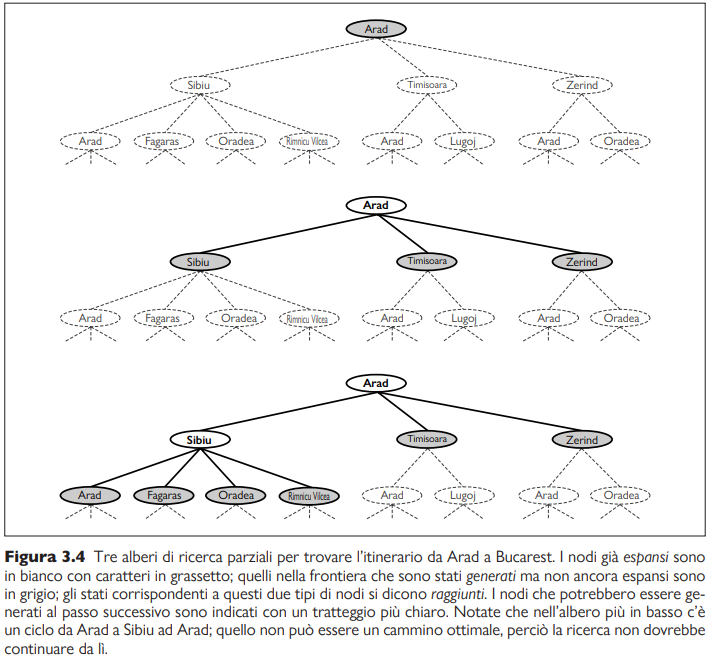
\includegraphics[width=0.5\linewidth]{Images/AlberiDiRicerca.png}
    \caption{Alberi di ricerca}
    \label{fig:enter-label}
\end{figure}
\par\noindent\rule{\textwidth}{0.4pt}
%Algoritmi di ricerca end
%Ricerca best-first start
\newpage
\subsubsection{Ricerca best-first}
Scegliamo un nodo n che corrisponde al valore minimo di una funzione di valutazione f(n). A ogni iterazione scegliamo un nodo sulla frontiera in cui f(n) ha valore minimo e lo restituiamo se il suo stato è uno stato obiettivo, altrimenti applichiamo ESPANDI per generare nodi figli. Ogni nodo figlio viene aggiunto alla frontiera se non è stato raggiunto in precedenza, o viene aggiunto di nuovo se è stato raggiunto con un cammino inferiore ai precedenti. L'algoritmo restituisce un indicatore di fallimento oppure un nodo che rappresenta un nodo che rappresenta un cammino che porta a un obiettivo.
%%%%%%%%%% RICERCA-BEST-FIRST start 
\begin{center}
\SetKwComment{Comment}{/* }{ */}
\begin{algorithm}
\caption{RICERCA-BEST-FIRST}
\KwData{problema, f}
\KwResult{\Return un nodo soluzione o fallimento;}
nodo$\leftarrow$NODO(STATO=problema.statoIniziale)\;
frontiera$\leftarrow$una coda con priorità ordinata in base a f, con nodo come elemento iniziale\;
raggiunti$\leftarrow$una tabella di lookuo, con un elemento con chiave problema.statoIniziale e valore nodo\;
\While{!frontiera.isEmpty()}{
nodo$\leftarrow$frontiera.pop()\;
\If{problema.è-obiettivo(nodo.STATO)}{
\Return nodo\;
}
\For{figlio \textbf{in} \textit{\textbf{ESPANDI}}(problema, nodo)}{
s$\leftarrow$figlio.STATO\;
\If{s!=raggiunto || figlio.COSTO-CAMMINO < raggiunti[s].COSTO-CAMMINO}{
raggiunti[s]$\leftarrow$figlio\;
frontiera.add(figlio)\;
}
}
}
\Return fallimento;
\end{algorithm}
\end{center}
\newpage
\begin{center}
\SetKwComment{Comment}{/* }{ */}
\begin{algorithm}
\caption{ESPANDI}
\KwData{problema, nodo}
\KwResult{\textbf{yelds} nodi;}
s$\leftarrow$nodo.STATO\;
\For{azione \textbf{in} problema.AZIONI(s)}{
s'$\leftarrow$problema.RISULTATO(s, azione)\;
costo$\leftarrow$nodo.COSTO-CAMMINO + problema.COSTO-AZIONE(s, azione, s')\;
\textbf{yeld} NODO(STATO=s',PADRE=nodo,AZIONE=azione,COSTO-CAMMINO=costo)\;
}
\end{algorithm}
\end{center}
\par\noindent\rule{\textwidth}{0.4pt}
%%%%%%%%%% RICERCA-BEST-FIRST end
%Ricerca best-first end
%Strutture dati per la ricerca start
\newpage
\subsubsection{Strutture dati per la ricerca}
Un nodo n nell'albero di ricerca è rappresentato da una struttura dati con quattro componenti:
\begin{itemize}
    \item \textbf{n.STATO}: lo stato a cui corrisponde il nodo;
    \item \textbf{n.PADRE}: il nodo dell'albero di ricerca che ha generato il nodo corrente;
    \item \textbf{n.AZIONE}: l'azione applicata allo stato del padre per generare il nodo corrente;
    \item \textbf{n.COSTO-CAMMINO}: il costo totale del cammino che va dallo stato iniziale al nodo corrente (spesso indicato con g(nodo)).
\end{itemize}
\noindent Partendo da un nodo obiettivo seguendo i puntatori ai nodi PADRE possiamo trovare la soluzione.\newline
La struttura dati usata per memorizzare la frontiera è la coda con le seguenti operazioni:
\begin{itemize}
    \item VUOTA?(frontiera): restituisce True se è vero altrimenti False.
    \item POP(frontiera): rimuove il nodo in cima alla frontiera e lo restituisce.
    \item TOP(frontiera): restituisce (senza rimuoverlo) il nodo in cima alla frontiera.
    \item AGGIUNGI(nodo, frontiera): inserisce un nodo al posto appropriato nella coda.
\end{itemize}
\noindent Negli algoritmi di ricerca si usano tre tipi di code:
\begin{itemize}
    \item \textbf{Coda di priorità}, in cui viene restituito il primo nodo di costo minimo in base a una funzione di valutazione f. Questo tipo di coda è usato nella ricerca best-first.
    \item \textbf{Coda FIFO}, in cui viene estratto il nodo che è stato inserito per primo. Usato nella ricerca BFS.
    \item \textbf{Coda LIFO}, ovvero lo Stack, in cui viene estratto l'ultimo nodo inserito. Usato nella ricerca DFS.
\end{itemize}
%Strutture dati per la ricerca end
%Cammini ridondanti start
\newpage
\subsubsection{Cammini ridondanti}
Un ciclo è un caso particolare di cammino ridondante. Il problema è che se l'algoritmo non riconosce un ciclo rischia di andare in loop. Ci sono tre approcci:
\begin{itemize}
    \item Il primo approccio consiste nel ricordare tutti gli stati precedentemente raggiunti, il che ci consente di individuare tutti i cammini ridondanti e mantenere soltanto il cammino migliore per raggiungere ogni stato.
    \item Il secondo approccio consiste nel non preoccuparsi di ripetere il passato. Esistono alcune formulazioni di problemi dove è impossibile che due cammini conducano allo stesso stato.
    \item Il terzo approccio è un compromesso: controlliamo la presenza di cammini ciclici, ma non di cammini ridondanti. Per evitare di usare memoria aggiuntiva, possiamo risalire alla catena di puntatori padre e vedere se lo stato al termine del cammino è già apparso in precedenza.
\end{itemize}
%Cammini ridondanti end
%Misurare le prestazioni nella soluione di problemi start
\newpage
\subsubsection{Misurare le prestazioni nella risoluzione di problemi}
Possiamo valutare le prestazioni di un algoritmo secondo 4 parametri:
\begin{itemize}
    \item Completezza: l'algoritmo consente di trovare tutte le soluzioni se esistono, o riportare il fallimento se non esistono?
    \item Ottimale rispetto al costo: trova la soluzione con il costo di cammino minimo fra tutte?
    \item Complessità temporale: quanto tempo impiega a trovare una soluzione?
    \item Costo spaziale: di quanta memoria necessita?
\end{itemize}
%Misurare le prestazioni nella soluione di problemi end
%Strategie di ricerca non informata start
\newpage
\subsection{Strategie di ricerca non informata}
Un algoritmo non informato non riceve alcuna informazione su quanto uno stato sia vicino all'obiettivo.
%Strategie di ricerca non informata end
%Ricerca in ampiezza start
\subsubsection{Ricerca in ampiezza, BFS}
Si tratta di una ricerca sistematica, completa anche su spazi a stati infiniti; si usa quando tutte le azioni hanno lo stesso costo. Si parte dalla radice, per poi visitare tutti i suoi successori e così via.
Può essere implementata come RICERCA-BEST-FIRST con f(n) uguale alla profondità del nodo, ovvero il numero di azioni necessarie per raggiungerlo. Invece della coda di priorità usiamo una coda FIFO che sarà più efficiente. \textbf{\textit{raggiunti}} sarà un insieme di stati visto che non ci interessa mantenere l'informazione del nodo non potendo più trovare un cammino migliore. La ricerca in ampiezza trova sempre la soluzione con minor numero di azioni visto che quando genera nodi di profondità d ha già generato nodi di profondità d-1, perciò se uno di essi fosse una soluzione sarebbe già stata trovata. Il numero totale di nodi generati per una soluzione di profondità d dove ogni nodo ha b successori è $O(b^d )$  che è la complessità spazio-temporale visto che tutti i nodi rimangono in memoria.
%%%%%%%%%% RICERCA-IN-AMPIEZZA start 
\begin{center}
\SetKwComment{Comment}{/* }{ */}
\begin{algorithm}
\caption{RICERCA-IN-AMPIEZZA}
\KwData{problema, f}
\KwResult{\Return un nodo soluzione o fallimento;}
nodo$\leftarrow$NODO(problema.STATOINIZIALE)\;
\If{problama.è-obiettivo(nodo.STATO)}{
\Return nodo\;
}
frontiera$\leftarrow$una coda FIFO, con nodo come elemento iniziale\;
raggiunti$\leftarrow$\{problema.STATOINIZIALE\}\;
\While{!frontiera.isEmpty()}{
nodo$\leftarrow$frontiera.pop()\;
\For{figlio \textbf{in} \textit{\textbf{ESPANDI}}(problema, nodo)}{
s$\leftarrow$figlio.STATO\;
\If{problema.è-obiettivo(s)}{
\Return figlio\;
}
\If{s!=raggiunto}{
raggiunti.add(figlio)\;
frontiera.add(figlio)\;
}
}
}
\Return fallimento;
\end{algorithm}
\end{center}
%%%%%%%%%% RICERCA-IN-AMPIEZZA end
%Ricerca in ampiezza end
%Algoritmo di Dijkstra o ricerca a costo uniforme start
\newpage
\subsubsection{Algoritmo di Dijkstra o ricerca a costo uniforme}
Quando le azioni hanno costi differenti si può usare la ricerca best-first con COSTO-CAMMINO come funzione di valutazione. La ricerca a costo uniforme, a differenza della ricerca in ampiezza che si diffonde a ondate di profondità uniforme, si diffonde a ondate di costo uniforme. La complessità della ricerca a costo uniforme è caratterizzata in termini di C*, il costo della soluzione ottima, ed $\epsilon >0$, un limite inferiore imposto al costo di ogni azione. Quindi, nel caso peggiore la complessità temporale e spaziale dell'algoritmo è data da $O(b^{1+\lfloor C^*/\epsilon \rfloor})$, che può essere molto maggiore di $O(b^d)$.\newline
La ricerca a costo uniforme è completa e ottima rispetto al costo, perché la prima soluzione che trova avrà un costo basso almeno quanto quello di ogni altro nodo sulla frontiera.
%%%%%%%%%% RICERCA-IN-UNIFORME start 
\begin{center}
\SetKwComment{Comment}{/* }{ */}
\begin{algorithm}
\caption{RICERCA-IN-UNIFORME}
\KwData{problema}
\KwResult{\Return un nodo soluzione o fallimento;}
\Return RICERCA-BEST-FIRST(problema, COSTO-CAMMINO)\;
\end{algorithm}
\end{center}
%%%%%%%%%% RICERCA-IN-UNIFORME end
%Algoritmo di Dijkstra o ricerca a costo uniforme end
%Ricerca in profondità e problema della memoria start
\newpage
\subsubsection{Ricerca in profondità e problema della memoria}
La ricerca in profondità espande sempre il nodo con profondità maggiore nella frontiera. Può essere implementata come una ricerca best-first con f opposto negativo della profondità.
Per spazi a stati finiti che sono alberi, la ricerca in profondità è efficace e completa; se sono presenti cicli, la ricerca in profondità può bloccarsi in un loop. Per i problemi che necessitano una ricerca ad albero, la ricerca in profondità ha esigenze di memoria molto più ridotte rispetto alle altre ricerche.
Per uno spazio degli stati finito e a forma di albero, la ricerca in profondità richiede memoria $O(bm)$ dove b è il fattore di ramificazione e m la massima profondità dell'albero.
%Ricerca in profondità e problema della memoria end
%Ricerca in profondità limitata e ad approfondimento iterativo start
\subsubsection{Ricerca in profondità limitata e ad approfondimento iterativo}
Per evitare che la ricerca in profondità si perda in un cammino infinito, possiamo usare la ricerca a profondità limitata, dove poniamo un limite \textit{l} e consideriamo tutti i nodi con profondità \textit{l} come se non avessero successori.
La complessità temporale è $O(b^l)$, quella spaziale è $O(bl)$. Questa ricerca è corretta a patto che si scelga correttamente \textit{l}.
La ricerca ad approfondimento iterativo, risolve il problema di trovare un buon valore di l\textit{} provando tutti i valori fino a trovare una soluzione oppure fino a riportare un fallimento. I costi di memoria sono $O(bd)$ quando esiste una soluzione, $O(bm)$ quando non esiste. I costi temporali sono $O(b^d)$ quando esiste una soluzione, $O(b^m)$ quando non esiste.
%%%%%%%%%% RICERCA-APPROFONDIMENTO-ITERATIVO start 
\begin{center}
\SetKwComment{Comment}{/* }{ */}
\begin{algorithm}
\caption{RICERCA-APPROFONDIMENTO-ITERATIVO}
\KwData{problema}
\KwResult{\Return un nodo soluzione o fallimento;}
\For{profondità = 0 \textbf{to} $\infty$}{
risultato$\leftarrow$RICERCA-PROFONDITÀ-LIMITATA(problema, profondità)\;
\If{risultato $!=$ soglia}{
\Return risultato\;
}
}
\end{algorithm}
\end{center}
%%%%%%%%%% RICERCA-APPROFONDIMENTO-ITERATIVO end
%%%%%%%%%% RICERCA-PROFONDITÀ-LIMITATA start 
\begin{center}
\SetKwComment{Comment}{/* }{ */}
\begin{algorithm}
\caption{RICERCA-PROFONDITÀ-LIMITATA}
\KwData{problema, l}
\KwResult{\Return un nodo soluzione o fallimento o soglia;}
frontiera$\leftarrow$ uno stack con NODO(problema.STATOINIZIALE) come elemento iniziale\;
risultato$\leftarrow$fallimento\;
\While{!frontiera.isEmpty()}{
nodo$\leftarrow$frontiera.pop()\;
\If{problema.È-OBIETTIVO(nodo.STATO}{
\Return nodo\;
}
\If{PROFONDITÀ(nodo)>l}{
risultato$\leftarrow$soglia\;
}\Else{
\If{nodo non ha un ciclo}{
\For{figlio \textbf{in} ESPANDI(problema, nodo)}{
frontiera.add(figlio)\;
}
}
}
}
\Return risultato\;
\end{algorithm}
\end{center}
%%%%%%%%%% RICERCA-PROFONDITÀ-LIMITATA end
%Ricerca in profondità limitata e ad approfondimento iterativo end
%Ricerca bidirezionale start
\newpage
\subsubsection{Ricerca bidirezionale}
Al contrario delle ricerche precedenti che partono da uno stato iniziale per raggiungere uno stato obiettivo, la ricerca bidirezionale procede simultaneamente partendo dallo state iniziale e dallo stato obiettivo (o stati obiettivi) nella speranza che le due ricerche si incontrino. L'idea è che il costo $b^{d/2}+b^{d/2}<<b^d$. Affinche questa strategia funzioni, è necessario tenere traccia di due frontiere e due tabelle di stati raggiunti, bisogna saper riconoscere che: se s' è successore di s nella tabella degli stati in avanti, allora s è successore di s' nella tabella degli stati in indietro. 
%%%%%%%%%% RICERCA-BEST-FIRST-BIDIREZIONALE start 
\begin{center}
\SetKwComment{Comment}{/* }{ */}
\begin{algorithm}
\caption{RICERCA-BEST-FIRST-BIDIREZIONALE}
\KwData{$problema_F,f_F,problema_B,f_B$}
\KwResult{\Return un nodo soluzione o fallimento;}
$nodo_F\leftarrow NODO(problema_F,STATOINIZIALE)$\;
$nodo_B\leftarrow NODO(problema_B,STATOINIZIALE)$\;
$frontiera_F\leftarrow \text{coda con priorità ordinata in base a }f_F,\text{ con }nodo_F \text{ come elemento iniziale}$\;
$frontiera_B\leftarrow \text{coda con priorità ordinata in base a }f_F,\text{ con }nodo_B \text{ come elemento iniziale}$\;
$raggiunti_F\leftarrow \text{tabella di lookup, con un elemento con chiave }nodo_F.\text{STATO e valore }nodo_F$\;
$raggiunti_B\leftarrow \text{tabella di lookup, con un elemento con chiave }nodo_B.\text{STATO e valore }nodo_B$\;
soluzione$\leftarrow fallimento$\;
\While{$!TERMINATO(soluzione,frontiera_F,frontiera_B)$}{
\If{$f_F(TOP(frontiera_F))<f_B(TOP(frontiera_B))$}{
    soluzione$\leftarrow PROCEDI(F,problema_F,frontiera_F,raggiunti_F,raggiunti_B,soluzione);$
}\Else{
soluzione$\leftarrow PROCEDI(B,problema_B,frontiera_B,raggiunti_B,raggiunti_F,soluzione);$
}
}
\Return soluzione\;
\end{algorithm}
\end{center}
%%%%%%%%%% RICERCA-BEST-FIRST-BIDIREZIONALE end
%%%%%%%%%% PROCEDI start 
\begin{center}
\SetKwComment{Comment}{/* }{ */}
\begin{algorithm}
\caption{PROCEDI}
\KwData{$dir, problema, frontiera, raggiunti, raggiunti_2, soluzione$}
\KwResult{\Return una soluzione}
\Comment{Espande nodo su frontiera; controlla rispetto all'altra frontiera in $raggiunti_2$\newline 
La variabile "dir" è la direzione: F per avanti o B per indietro.}
$nodo\leftarrow frontiera.pop()$\;
\For{figlio \textbf{in} ESPANDI(problema, nodo)}{
s$\leftarrow$figlio.STATO\;
\If{!raggiunti.contains(s) || COSTO-CAMMINO(figlio) < COSTO-CAMMINO(raggiunti[s])}{
raggiunti[s]$\leftarrow$figlio\;
aggiungi figlio a frontiera\;
\If{$raggiunti_2$.contains(s)}{
$soluzione_2\leftarrow$UNISCI-NODI(dir,figlio,$raggiunti_2[s]$)\;
\If{COSTO-CAMMINO($soluzione_2$<COSTO-CAMMINO(soluzione)}{
soluzione$\leftarrow soluzione_2$\;
}
}
}
}
\Return soluzione\;
\end{algorithm}
\end{center}
%%%%%%%%%% PROCEDI end

%Ricerca bidirezionale end
%Confronto tra le strategie di ricerca non informata start
\subsubsection{Confronto tra le strategie di ricerca non informata}
\begin{figure}[H]
    \centering
    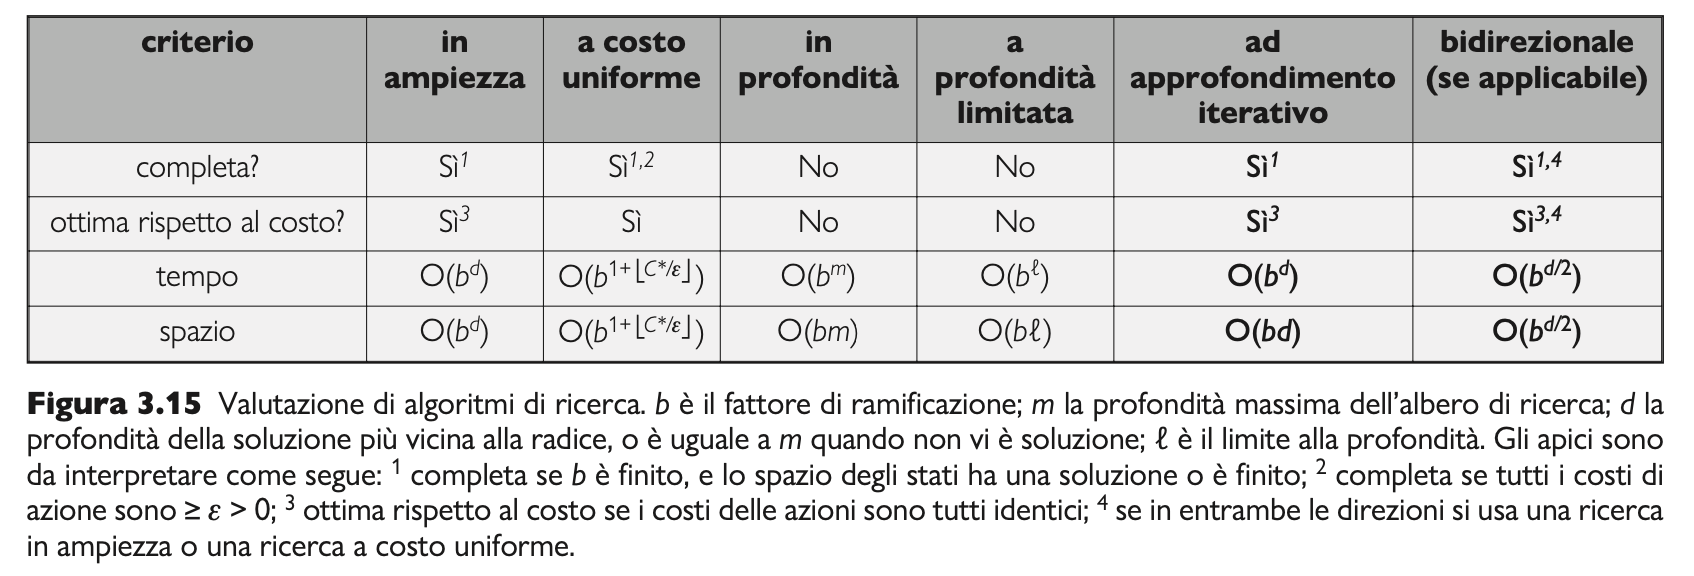
\includegraphics[width=0.5\linewidth]{Images/ValutazioneAlgoritmmiRicercaNonInformata.png}
    \caption{Valutazione Strategie di ricerca non informata}
    \label{fig:enter-label}
\end{figure}
Tale confronto riguarda le versioni di ricerca ad albero senza controllo di stati ripetuti. Per le ricerche su grafo che effettuano tale controllo, le differenze principali sono che la ricerca in profondità è completa per spazi degli stati finiti e che le complessità spaziale e temporale sono limitate dalla dimensione dello spazio degli stati (il numero di vertici e archi, $|V| + |E|$).
%Confronto tra le strategie di ricerca non informata end
%Strategie di ricerca informata o euristica start
\newpage
\subsection{Strategie di ricerca informata o euristica}
La ricerca informata sfrutta conoscenza specifica del dominio applicativo per fornire suggerimenti su dove si potrebbe trovare l'obiettivo per trovare soluzioni in modo più efficiente di una strategia non informata. I suggerimenti che passiamo hanno la forma di funzione euristica denotata con 
h(n) = costo stimato del cammino meno costoso dallo stato del nodo n a uno stato obiettivo.
%Strategie di ricerca informata o euristica end
%Ricerca best-first greedy o “golosa” start
\subsubsection{Ricerca best-first greedy o “golosa”}
La ricerca best-first greedy (BFG) è come una ricerca best-first che espande prima il nodo con il valore più basso di $h(n)$, cioè quello più vicino all'obiettivo, sulla base del fatto che è probabile che questo porti rapidamente a una soluzione. Questo implica che la funzione di valutazione $f(n) = h(n)$. La ricerca BFG su un grafo è completa negli spazi degli stati finiti, ma non in quelli infiniti. Nel caso peggiore la complessità temporale e spaziale è $O(|V|)$, ma con una buona funzione euristica si arriva a $O(bm)$.
%Ricerca best-first greedy o “golosa” end
%Ricerca A* start
\subsubsection{Ricerca $A^*$}
La forma più diffusa di algoritmo di ricerca informata è la ricerca $A^*$, un ricerca best-first che utilizza la funzione di valutazione: $f(n) = g(n) +h(n)$, dove g(n) è il costo del cammino dal nodo iniziale al nodo n e h(n) rappresenta il costo stimato del cammino più breve da n a uno stato obiettivo, per cui abbiamo:
F(n) = costo stimato del cammino migliore che continua da n fino a un obiettivo. La ricerca $A^*$ è completa, l'ottimalità rispetto al costo dipende da alcune proprietà:
\begin{enumerate}
    \item \textbf{Ammissibilità}: un'euristica ammissibile è tale se non sovrastima mai il costo per raggiungere un obiettivo ( si dice ottimista). Con un euristica ammissibile la ricerca A* è ottima rispetto al costo; dimostrazione per assurdo:
    Supponiamo che il cammino ottimo abbia costo $C^*$, ma l'algoritmo restituisca un cammino di costo maggiore: $C>C^*$. Allora deve esistere un nodo n che si trova sul cammino ottimo e non è espanso (altrimenti sarebbe stata restituita la soluzione ottima). Allora, sia $g^*(n)$ il costo del cammino ottimo dall'inizio a n e con $h^*(n)$ il costo del cammino ottimo da n fino all'obiettivo più vicino:\newline
    {%
    \centering
    $f(n)>C^*$\newline
    $F(n)=g(n)+h(n)$\newline
    $F(n)=g^*(n)+h(n)$\newline
    $F(n)\leq g^*(n)+h^*(n)$\newline
    $F(n)\leq C^* $\newline
    }
    La prima e l'ultima riga si contraddicono, quindi l'ipotesi è errata e A* deve restituire soltanto cammini ottimi rispetto al costo.
    \item Consistenza: un'euristica h(n) è consistente se, per ogni nodo n e ogni successore n' di n generato da un'azione a, abbiamo: $h(n\leq c(n, a, n')+h(n')$. Questa è una forma di disuguaglianza triangolare, per cui ogni lato di un triangolo non può essere più lungo della somma degli altri due. Ogni euristica consistente è ammissibile (ma non vale il vice versa), perciò $A^*$ con un'euristica consistente è ottima rispetto al costo. Inoltre, con un'euristica consistente, la prima volta che raggiungiamo uno stato sarà su un cammino ottimo, perciò non dovremo mai aggiungere di nuovo uno stato alla frontiera, né dovremo mai modificare un elemento in raggiunti. Con un euristica inconsistente, potremmo ritrovarci con più cammini che raggiungono lo stesso stato, e se ogni cammino nuovo ha un costo inferiore al precedente, finiremo con l'avere più nodi corrispondenti a quello stato sulla frontiera, con un aggravio di costo temporale e spaziale.
\end{enumerate}

\noindent Con un euristica inammissibile, $A^*$ può essere ottima rispetto al costo oppure no. Di seguito due casi in cui lo è: 
\begin{enumerate}
    \item Se vi è anche un solo cammino ottimo rispetto al costo lungo cui h(n) è ammissibile per tutti i nodi n sul cammino, allora tale cammino verrà trovato a prescindere da quanto affermi l'euristica per gli stati al di fuori di esso. 
    \item Se la soluzione ottima ha un costo $C^*$ e la seconda migliore ha un costo $C_2$, e se h(n) sovrastima alcuni costi, ma mai più di $C_2-C^*$, allora $A^*$ restituisce sempre soluzioni ottime rispetto al costo.
\end{enumerate}
%Ricerca A* end
%Confini di ricerca start
\newpage
\subsubsection{Confini di ricerca}
Quando si estende un cammino, i costi g sono monotoni: il costo del cammino aumenta sempre mentre lo si percorre, poiché i costi di azione sono sempre positivi. \newline
Sia $C^*$ il costo del cammino nella soluzione ottima, possiamo dire:
\begin{itemize}
    \item $A^*$ espande tutti i nodi che possono essere raggiunti dallo stato iniziale su un cammino in cui per ogni nodo si ha f(n) < $C^*$. Questi sono nodi certamente espansi.
    \item $A^*$ potrebbe poi espandere alcuni dei nodi proprio sul "confine obiettivo" prima di selezionare un nodo obiettivo.
    \item $A^*$ non espande alcun nodo con $f(n)>C^*$.
\end{itemize}
Diciamo che $A^*$ con euristica consistente è ottimamente efficiente nel senso che qualsiasi algoritmo che estende cammini di ricerca a partire dallo stato iniziale e usa la stessa euristica deve espandere tutti i nodi che sono certamente espansi da $A^*$.\newline
$A^*$ è efficiente perché esegue la potatura dell'albero di ricerca dei nodi non necessari per trovare una soluzione ottima.
%Confini di ricerca end
%Ricerca soddisfacente: euristiche inammissibili e ricerca A* pesata start
\newpage
\subsubsection{Ricerca soddisfacente: euristiche inammissibili e ricerca $A^*$ pesata}
Se si è disposti ad accettare soluzioni subottime ma "sufficientemente buone", soddisfacenti, possiamo migliorare la ricerca $A^*$ facendo espandere un minor numero di nodi. Se consentiamo alla ricerca $A^*$ di usare un'euristica inammissibile rischiamo di non trovare una soluzione ottima, ma l'euristica potrebbe essere più accurata, riducendo così il numero di nodi espansi.
Con una ricerca $A^*$ pesata possiamo dare peso maggiore al valore dell'euristica, con la funzione di valutazione $f(n)=g(n)+Wh(n)$ con $W > 1$. La ricerca pesata focalizza il confine degli stati raggiunti verso un obiettivo: ciò significa che vengono esplorati meno stati, ma se il cammino ottimo va al di fuori del confine, il cammino ottimo non viene trovato. Il costo della soluzione ottima della ricerca A* pesata è compreso tra $C^*$ e $WC^*$. La ricerca $A^*$ pesata può essere considerata una generalizzazione delle altre; esistono vari tipi di algoritmi di ricerca subottimali:
\begin{itemize}
    \item \textbf{Ricerca a subottimalità limitata}: cerchiamo una soluzione per cui vi sia la garanzia che si trovi entro un fattore costante W del costo ottimo.
    \item \textbf{Ricerca a costo limitato}: cerchiamo una soluzione il cui costo sia inferiore a una costante C.
    \item \textbf{Ricerca a costo illimitato}: accettiamo una soluzione di qualsiasi costo, purché riusciamo a trovarla rapidamente.
\end{itemize}
%Ricerca soddisfacente: euristiche inammissibili e ricerca A* pesata end
%Ricerca con memoria limitata start
\newpage
\subsubsection{Ricerca con memoria limitata}
La principale problematica della ricerca $A^*$ è legata all'impiego di memoria che è suddiviso tra la frontiera e gli stati raggiunti. Una ridondanza nell'implementazione della ricerca best-first è legata al fatto che lo stato che si trova sulla frontiera è memorizzato in due posizioni: come nodo della frontiera e come elemento nella tabella degli stati raggiunti.\newline
La \textbf{ricerca beam} limita la dimensione della frontiera. L'approccio più semplice consiste nel mantenere soltanto i k nodi con i migliori costi f, scartando ogni altro nodo espanso; questo rende la ricerca incompleta e subottima, ma possiamo scegliere k per fare buon uso della memoria disponibile, e l'algoritmo viene eseguito velocemente perché espande meno nodi. \newline
Mentre la ricerca a costo uniforme e la ricerca $A^*$ si espandono in confini concentrici, la ricerca beam esplora soltanto un settore di tali confini, il "fascio" che contiene i k migliori candidati.\newline
La \textbf{ricerca $A^*$ ad approfondimento iterativo ($IDA^*$)} sta alla ricerca $A^*$ come la ricerca ad approfondimento iterativo sta alla ricerca in profondità: la ricerca IDA* fornisce i vantaggi della ricerca $A^*$ senza la necessità di mantenere in memoria tutti gli stati raggiunti, al costo di vistare alcuni stati più volti. Nella ricerca approfondimento iterativo standard la soglia è la profondità, che aumenta a ogni iterazione; nella ricerca $IDA^*$ la soglia è il costo $f(g+h)$; a ogni iterazione il valore soglia p il più piccolo costo f di qualsiasi nodo che abbia superato la soglia nella precedente iterazione.\newline
La \textbf{ricerca best-first ricorsiva (RBFS)} tenta di imitare il funzionamento di una ricerca best-first standard usando solamente uno spazio lineare.  L'algoritmo usa una variabile f\_limite per tenere traccia il valore f del miglior cammino alternativo che parte da uno qualsiasi degli antenati del nodo corrente. Se il nodo supera il limite, la ricorsione torna indietro al cammino alternativo. Durante il ritorno, RBFS sostituisce il valore f di ogni nodo lungo il cammino con un valore di backup, il miglior valore f dei suoi nodi figli.  In questo modo RBFS ricorda il valore f della foglia migliore nel sottoalbero abbandonato e può quindi decidere in seguito di ri-espanderlo. \newline
%%%%%%%%%% RICERCA-BEST-FIRST-RICORSIVA start 
\begin{center}
\SetKwComment{Comment}{/* }{ */}
\begin{algorithm}
\caption{RICERCA-BEST-FIRST-RICORSIVA}
\KwData{$problema$}
\KwResult{\Return una soluzione o fallimento}
$soluzione,valoref\leftarrow RBFS(problema, NODO(problema.STATOINIZIALE),\infty)$\;
\Return $soluzione$\;
\end{algorithm}
\newpage
\SetKwComment{Comment}{/* }{ */}
\begin{algorithm}
\caption{RBFS}
\KwData{$problema,nodo,f\_limite$}
\KwResult{\Return una soluzione o fallimento e il nuovo limite al costo f}
\If{problema.È\_OBIETTIVO(nodo.STATO)}{\Return nodo\;}
$successori\leftarrow LISTA(ESPANDI(nodo))$\;
\If{successori è vuoto}{\Return fallimento, $\infty$\;}
\For{s \textbf{in} successori}{$s.f\leftarrow max(s.COSTO\text{-}CAMMINO+h(s),nodo.f)$\;}
\While{True}{$migliore\leftarrow \text{il nodo con valoref minimo in }successori$\;
\If{migliore.f>f\_limite}{\Return fallimento, migliore.f\;}
$alternativa\leftarrow \text{il secondo nodo con valore valoref minimo tra }successori$\;
$risultato, migliore \leftarrow RBFS(problema, migliore, min(f\_limite,alternativa))$\;
\If{$risultato\neq fallimento$}{\Return risultato, migliore.f\;}
}
\end{algorithm}
\end{center}
%%%%%%%%%% RICERCA-BEST-FIRST-RICORSIVA end
RBFS è un algoritmo ottimo se la funzione euristica h(n) è ammissibile. La sua complessità spaziale è lineare nella profondità della più profonda soluzione ottimale, ma quella temporale è abbastanza difficile da definire, perché dipende sia dall'accuratezza della funzione euristica sia dalla frequenza dei cambiamenti del cammino ottimale durante l'espansione dei nodi. L'algoritmo RBFS espande i nodi in ordine crescente di costo f anche se f non è monotona.\newline
Il problema degli algoritmi $IDA^*$ e RBFS è che usano troppo poca memoria.
Poiché entrambi gli algoritmi dimenticano la maggior parte di ciò che hanno fatto, potrebbero riesplorare nuovamente gli stessi stati molte volte. È quindi importante determinare quanta memoria è disponibile e consentire all'algoritmo di utilizzarla; ci sono due algoritmi che lo fanno: \textbf{$MA^*$ (memory-bounded $A^*$)} e \textbf{$SMA^*$ (simplified $MA^*$)}. Verrà analizzato solo $SMA^*$.\newline
\textbf{$SMA^*$} procede proprio come $A^*$, espandendo la foglia migliore finché la memoria è piena. A questo punto non può aggiungere un nuovo nodo all'albero di ricerca senza cancellarne uno vecchio. $SMA^*$ scarta sempre il nodo foglia peggiore, quello con costo f più alto. Come RBFS, memorizza nel nodo padre il valore del nodo dimenticato. In questo modo la radice di un sottoalbero dimenticato conosce la qualità del cammino migliore in quel sottoalbero. Con quest'informazione $SMA^*$ ri-genera il sottoalbero dimenticato solo quando tutti gli altri cammini promettono di comportarsi peggio di quello. Potremmo anche dire che, se tutti i discendenti di un nodo n sono dimenticati, allora non sappiamo da che parte andare partendo da n, ma abbiamo ancora un'idea chiara di quanto sia conveniente passare per n.\newline
L'algoritmo $SMA^*$ è completo se c'è una soluzione raggiungibile, ovvero se d, la profondità del nodo obiettivo più vicino alla radice, è inferiore alla dimensione della memoria espressa in nodi. La strategia è ottima se c'è una soluzione ottima raggiungibile; altrimenti viene restituita la soluzione migliore tra quelle raggiungibili.
%Ricerca con memoria limitata end
%Ricerca euristica bidirezionale start
\newpage
\subsubsection{Ricerca euristica bidirezionale}
Nel caso della ricerca best-first unidirezionale usando f(n)=g(n)+h(n) si ottiene la ricerca $A^*$. Usando lo stesso f(n) nel caso della ricerca best-first bidirezionale non vi è garanzia di una soluzione ottima, né che la ricerca sia ottimamente efficiente, anche con un'euristica ammissibile.
Introduciamo ora una nuova notazione:
\begin{itemize}
    \item Sia $f_F (n)=g_F(n)+hF(n)$ per nodi nella direzione in avanti;
    \item Sia $f_B (n)=g_B(n)+hB(n)$ per nodi nella direzione all'indietro.
\end{itemize}

Le euristiche sono diverse visto che uno punta a trovare la soluzione e l'altro il nodo iniziale. Assumiamo euristiche ammissibili. Il costo di un cammino dallo stato iniziale a un nodo m e di un cammino all'indietro dall'obiettivo ad un nodo n deve essere almeno pari alla somma dei costi del cammino delle due parti e tale costo deve anche essere almeno pari al costo di f stimato di ciascuna delle due parti:
	$$lb(m,n)=max(g_F(m)+g_B(n),f_F(m),f_B(n)).$$
\begin{theorem}
Per ogni coppia di nodi (m, n) con lb(m, n) minore del costo ottimale C*, dobbiamo espandere m o n perché il cammino che passa per essi è potenzialmente una soluzione ottima.
\end{theorem}
\noindent La difficoltà sta nel scegliere quale nodo porta alla soluzione ottima. Noi passiamo all'algoritmo una funzione di valutazione che imita il criterio lb: $$f_2(n)=max(2g(n),g(n)+h(n))$$. Il nodo successivo da espandere è sempre quello che minimizza questo valore e può provenire da entrambe le frontiere. Questa funzione garantisce che non espanderemo mai un nodo con $g(n)>C^*/2$. 
In questo approccio $h_F$  stima la distanza dall'obiettivo e $h_B$ la distanza dall'inizio; in questo caso si parla di ricerca front-end. Un'alternativa è la ricerca front-to-front che cerca di stimare la distanza dall'altra frontiera.
%Ricerca euristica bidiirezionale end
%Funzioni euristiche start
\newpage
\subsection{Funzioni euiristiche}
Esempio funzioni euristiche su gioco dell'otto: 
Ci sono $9!/2$ stati raggiungibili in questo rompicapo perciò potrebbe benissimo mantenerli tutti in memoria, ma se aumentiamo il numero di caselle, ad esempio a 15, la cosa non è sostenibile. Ecco due delle euristiche più comuni:
\begin{itemize}
    \item h1= il numero di caselle fuori posto; è ammissibile perché ogni casella fuori posto richiederà almeno uno spostamento per farlo arrivare al posto giusto.
    \item h2=la somma delle distanze dei tasselli dalla loro posizione attuale alla posizione obiettivo. Dato che non si possono muovere in orizzontale la distanza è data dalla \textbf{distanza Manhattan}; è ammissibile perché ogni mossa può al massimo spostare la casella un passo più vicino al suo obiettivo.
\end{itemize}


%Funzioni euristiche end
%Cap. Risolvere i problemi con la ricerca end
\end{document}
%document end